\documentclass[12pt]{article}
\usepackage[margin = 1.5in]{geometry}
\setlength{\parindent}{0in}
\usepackage{amsfonts, amssymb, amsthm, mathtools, tikz, qtree, float}
\usepackage[lined]{algorithm2e}
\usepackage[T1]{fontenc}
\usepackage{ae, aecompl, color}
\usepackage[pdftex, pdfauthor={Charles Shen}, pdftitle={CS 251: Computer Organization and Design}, pdfsubject={Lecture notes from CS 251: Computer Organization and Design at the University of Waterloo}, pdfkeywords={CS 251, course notes, notes, Waterloo, University of Waterloo}, pdfproducer={LaTeX}, pdfcreator={pdflatex}]{hyperref}
\usepackage{cleveref}
\usepackage{wrapfig}
\usepackage{multicol, multirow}

\DeclarePairedDelimiter{\set}{\lbrace}{\rbrace}

\definecolor{darkish-blue}{RGB}{25,103,185}

\hypersetup{
  colorlinks,
  citecolor=darkish-blue,
  filecolor=darkish-blue,
  linkcolor=darkish-blue,
  urlcolor=darkish-blue
}

\theoremstyle{definition}
\newtheorem*{defn}{Definition}
\newtheorem*{theorem}{Theorem}
\newtheorem*{corollary}{Corollary}
\newtheorem{ex}{Example}[section]

\crefname{ex}{Example}{Example}

\setlength{\marginparwidth}{1.5in}
\newcommand{\lecture}[1]{
  \marginpar{{
    \footnotesize $\leftarrow$ \underline{#1}}
  }
}

\newcommand{\includePicture}[3]{
  \begin{figure}[!ht]
  \centering
  \scalebox{#1}{\includegraphics{#2}}
  \caption{#3}
  \end{figure}
}

\allowdisplaybreaks

\makeatletter
\def\blfootnote{\gdef\@thefnmark{}\@footnotetext}
\makeatother

%%%%%%%%%%%%%%%%%%%%%
%% D O C U M E N T %%
%%%%%%%%%%%%%%%%%%%%%

\begin{document}
  \let\ref\Cref

  \title{\bf{CS 251: Computer Organization and Design}}
  \date{Spring 2016, University of Waterloo \\ \center Notes written from Safaa Bedawi's lectures.}
  \author{Charles Shen}

  \blfootnote{Feel free to email feedback to me at
  \href{mailto:echen902@gmail.com}{echen902@gmail.com}.}

  \maketitle
  \newpage
  \tableofcontents
  \newpage

  \section{Performance}
  \subsection{Defining Performance}
  Performance can be defined in terms of more than just speed.
  Different performance metrics are required for different scenarios.
  To an individual, the performance in interest is \emph{response time}---the time between the start and completion of a task---also referred to as \emph{execution time}. \\
  To a data-center manager, the interest is in \emph{throughput} or \emph{bandwidth}---the total amount of work done in a given time.

  \subsection{Measuring Performance}
  Time is the measure of computer performance; the computer that performs the same amount of work in the least time is the fastest. \\
  Program execution time is measured in seconds per program, this is usually known as \emph{elapsed time, wall clock time, \emph{or} response time}. \\

  Computers are often shared, so a processor may work on several programs simultaneously.
  In which, the system attempts to optimize throughput rather than attempting to minimize the elapsed time for a program. \\

  The \emph{CPU execution time}, also knowns as \emph{CPU time}, makes the distinction between the elapsed time and the actual time the CPU spends computing for a specific task. \\
  Further distinction can be made, \emph{user CPU time}, the CPU time spent in the program, and \emph{system CPU time}, the CPU time spent in the operating system performing tasks on behalf of the program. \\

  Another measure of performance is using a measure that relates to how fast the hardware can perform basic functions. \\
  Almost all computers are constructed using a clock that determines when events take place in the hardware.
  These discrete time intervals are called \emph{clock cycles} (or ticks, clock ticks, clock periods, clocks, cycles). \\
  The length of a clock period can be either the time for a complete clock cycle (e.g. 250 picoseconds, or 250 ps) or the clock rate (e.g. 4 gigahertz, or 4GHz), which is the inverse of the clock period.
  $$1ps = 1 \times 10^{-12} = \frac{1}{1,000,000,000,000}$$

  \subsection{CPU Performance and Its Factors}
  \begin{align*}
  \parbox{4cm}{CPU execution time\\for a program}
  &= ~\parbox{3.5cm}{CPU clock cycles\\for a program} \times \text{ Clock cycle time} \\
  &= \frac{\text{CPU clock cycles for a program}}{\text{Clock rate}}
  \end{align*}

  \subsection{Instruction Performance}
  $$\text{CPU clock cycles} = ~\parbox{3cm}{Instructions for\\a program} \times ~\parbox{4cm}{Average clock cycles\\per instruction}$$
  \emph{Clock cycles per instruction}, which is the average number of clock cycles each instruction takes to execute, is often abbreviated as \emph{CPI}. \\
  CPI is an average of all the instructions executed in the program because different instructions may take different amounts of time depending on what they do.

  \subsection{The Classic CPU Performance Equation}
  $$\text{CPU time} = \text{Instruction count} \times \text{CPI} \times \text{Clock cycles time}$$
  Note that CPU varies by \emph{instruction mix}, which is a measure of the dynamic frequency of instructions across one or many programs.

  \section{From Zero To One, Abstractions}
  \includePicture{0.6}{pictures/abstractionLevel.png}{Levels of abstraction for electronic computing system}

  \subsection{The Three -Y's}
  \begin{itemize}
    \item [\textbf{Hierarchy}] involves dividing a system into modules, then further subdividing each of these modules until the pieces are easy to understand
    \item [\textbf{Modularity}] states that the modules have well-defined functions and interfaces, so that they connect together easily without unanticipated side effects
    \item [\textbf{Regularity}] seeks uniformity among the modules. Common modules are reused many times, reducing the number of distinct modules that must be designed
  \end{itemize}

  \subsection{Hexadecimal Number System}
  \begin{tabular} {c | c | c}
  Hexadecimal Digit & Decimal Digit & Binary Equivalent \\ \hline \hline
  0 & 0 & 0000 \\ \hline
  1 & 1 & 0001 \\ \hline
  2 & 2 & 0010 \\ \hline
  3 & 3 & 0011 \\ \hline
  4 & 4 & 0100 \\ \hline
  5 & 5 & 0101 \\ \hline
  6 & 6 & 0110 \\ \hline
  7 & 7 & 0111 \\ \hline
  8 & 8 & 1000 \\ \hline
  9 & 9 & 1001 \\ \hline
  A & 10 & 1010 \\ \hline
  B & 11 & 1011 \\ \hline
  C & 12 & 1100 \\ \hline
  D & 13 & 1101 \\ \hline
  E & 14 & 1110 \\ \hline
  F & 15 & 1111 \\
  \end{tabular}

  \subsection{Bytes, Nibbles, and All That Jazz}
  A group of eight bits is called a \emph{byte}. Represents $256 = 2^{8}$ possibilities. \\
  A group of four bits is called a \emph{nibble}. Represents $16 = 2^{4}$ possibilities. \\
  A microprocessor is a processor built on a single chip. \\
  Microprocessors handle data in chunks called words. The size of a word depends on the architecture of the microprocessor. \\
  Within a group of bits, the bit in the 1's column is called the least significant bit (lsb), and the bit at the other end is called the most significant bit (msb). \\
  Within a word, the bytes are identified as least significant byte (LSB) through most significant byte (MSB). \\

  \blfootnote{When adding operands with different signs, overflow cannot occur because the sum must be no larger than one of the operands.}
  \newpage

  \subsection{Logic Gates}
  A circuit element that performs a basic logic function \\ \\
  \textbf{Single Input} \\
  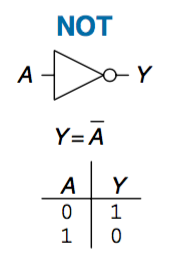
\includegraphics[scale=0.9]{pictures/notGate.png}
  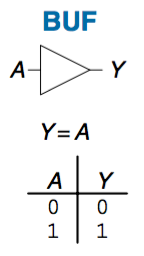
\includegraphics[scale=0.9]{pictures/bufGate.png} \\
  \textbf{Double Output} \\
  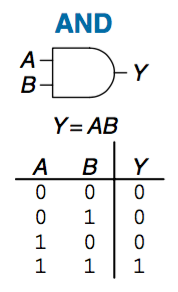
\includegraphics[scale=0.9]{pictures/andGate.png}
  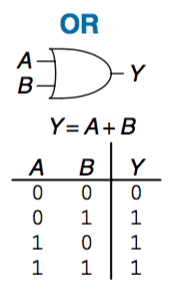
\includegraphics[scale=0.9]{pictures/orGate.png}
  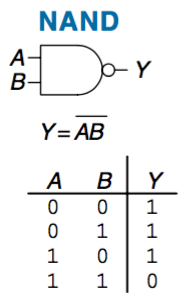
\includegraphics[scale=0.9]{pictures/nandGate.png}
  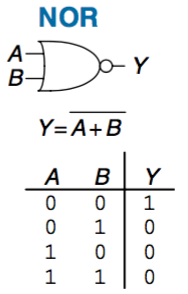
\includegraphics[scale=0.9]{pictures/norGate.png}
  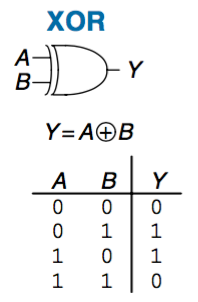
\includegraphics[scale=0.9]{pictures/xorGate.png}

  \subsection{Beneath the Digital Abstraction}
  A digital system uses discrete-valued variables. \\
  Variables are represented by continuous physical quantities such as the voltage on a wire, the position of a gear, or the level of fluid in a cylinder.
  \begin{ex}
    Consider representing a binary signal A with a voltage on a wire. \\
    Let 0 volts (V) indicate A = 0 and 5V indicate A = 1. \\
    Any real system must tolerate some noise, so 4.97V probably ought to be interpreted as A = 1 as well. \\
    But what about 4.3V? Or 2.8V? Or 2.5000000V?
  \end{ex}
  \subsubsection{Supply Voltage}
  Suppose the lowest voltage in the system is 0V, also called ground or GND \\
  The highest voltage in the system comes from the power supply and is usually called $V_{DD}$

  \subsubsection{Logic Levels}
  Mapping of a continuous variable onto a discrete binary variable is done by defining logic levels.
  First gate is called the driver and the second gate is called the receiver.
  Output of the driver is connected to the input of the receiver. \\
  The driver produces a LOW (0) output in the range of 0 to $V_{OL}$ or a HIGH (1) output in the range of $V_{OH}$ to $V_{DD}$

  \subsubsection{Noise Margins}
  If the output of the driver is to be correctly interpreted at the input of the receiver, we must choose $V_{OL} < V_{IL}$ and $V_{OH} > V_{IH}$ \\
  Even if the output of the driver is contaminated by some noise, the input of the receiver will still detect the correct logic level.
  Noise margin is the amount of noise that could be added to a worst-case output such that the signal can still be interpreted as a valid input

  \blfootnote{Note: power flows from drain to source.}

  \subsubsection{DC Transfer Characteristics}
  The DC transfer characteristics of a gate describe the output voltage as a function of the input voltage when the input is changed slowly enough that the output can keep up. \\
  Called transfer characteristics because they describe the relationship between input and output voltages.

  \section{CMOS Transistors}
  Transistors are electrically controlled switches that turn ON or OFF when a voltage or current is applied to a control terminal. \\
  Two main types of transistors are bipolar transistors and metal-oxide-semiconductor field effect transistors (MOSFETs or MOS transistors).

  \subsection{Semiconductors}
  MOS transistors are built from silicon. \\
  Silicon has four electrons in its valence shell and forms bonds with four adjacent atoms, resulting in a crystalline lattice. \\
  By itself, silicon is a poor conductor due to all the electrons are tied up in covalent bonds. \\
  Becomes a better conductor when small amounts of impurities, called dopant atoms, are added. \\
  The conductivity of silicon changes over many orders and of magnitude depending on the concentration of dopants, silicon is called a semiconductor. \\
  \textbf{Add Arsenic} \\
  If arsenic (As), a group V dopant, is added, the dopant atoms have an extra electron that is not involved in the bonds. \\
  Electron can easily move about the lattice, leaving an ionized dopant atom (As+) behind. \\
  Electron carries a negative charge, so arsenic is an n-type dopant. \\
  \textbf{Add Boron} \\
  If boron (B), a group III dopant, is added, the dopant atoms are missing an electron. \\
  The missing electron is called a hole. \\
  An electron from a neighboring silicon atom may move over to fill the missing bond, forming an ionized dopant atom (B-) and leaving a hole at the neighboring silicon atom. \\
  The hole can migrate around the lattice. \\
  Hole is a lack of negative charge, so it acts like a positively charged particle. \\
  So boron is a p-type dopant.

  \subsection{Diodes}
  \begin{wrapfigure}{r}{0.25\textwidth}
    \centering
    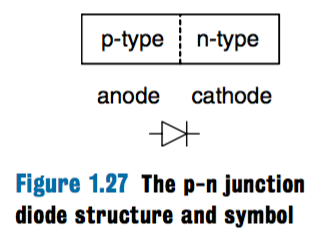
\includegraphics[width=0.25\textwidth]{pictures/diode.png}
  \end{wrapfigure}
  Junction between p-type and n-type silicon is called a diode.
  The p-type region is called the anode and the n-type region is called the cathode. \\
  When the voltage on the anode rises above the voltage on the cathode, the diode is forward biased, and current flows through the diode from the anode to the cathode. \\
  When the anode voltage is lower than the voltage on the cathode, the diode is reverse biased, and no current flows. \\
  The diode symbol intuitively shows that current only flows in one direction.

  \subsection{Capacitors}
  A \emph{capacitor} consists of two conductors separated by an insulator. \\
  When a voltage $V$ is applied to one of the conductors, the conductor accumulates electric \emph{charge} $Q$ and the other conductor accumulates the opposite charge $-Q$. \\
  The \emph{capacitance} C of the capacitor is the ratio of charge to voltage: $C = \frac{Q}{V}$.
  The capacitance is proportional to the size of the conductors and inversely proportional the distance between them. \\
  Capacitance is important because charing or discharging a conductor takes time and energy. More capacitance means that a circuit will be slower and require more energy to operate.

  \subsection{nMOS and pMOS Transistors}
  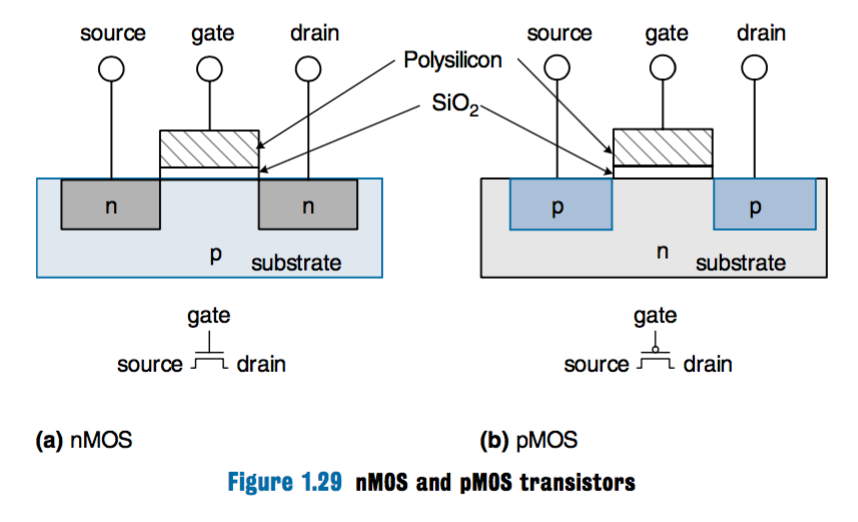
\includegraphics{pictures/nMOSpMOS.png} \\
  A MOSFET is a sandwich of several layers of conducting and insulating materials. \\
  There are two flavors of MOSFETs: nMOS and pMOS. \\
  The n-type transistors, called \emph{nMOS}, have regions of n-type dopants adjacent tot he gate called the \emph{source} and the \emph{drain} and are built on a p-type semiconductor substrate. \\
  The \emph{pMOS} transistors are just the opposite, consisting of p-type source and drain regions in an n-type \emph{substrate}. \\
  A MOSFET behaves as a voltage-controlled switch in which the gate voltage creates an electric field that turns ON or OFF a connection between the source and drain. \\
  nMOS transistors pass 0's well but passes 1's poorly.
  Similarly, pMOS transistors pass 1's well but 0's poorly. \\
  nMOS transistors need a p-type substrate, and pMOS transistors need an n-type substrate.
  To build both flavors of transistors on the same chip, manufacturing processes typically start with a p-type wafer, then implant n-type region called wells where the pMOS transistors should go.
  These processes that provide both flavors of transistors are called Complementary MOS or CMOS.
  \begin{wrapfigure}{r}{0.5\textwidth}
    \centering
    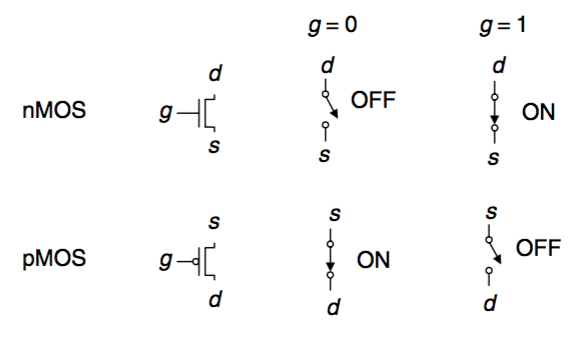
\includegraphics[width=0.5\textwidth]{pictures/nMOSpMOSGate.png}
  \end{wrapfigure}
  CMOS processes are used to build the vast majority of all transistors fabricated today. \\
  CMOS processes provide two types of electrically controlled switches.
  nMOS transistors are OFF when the gate is 0 and ON when the gate is 1.
  pMOS transistors are just the opposite: ON when the gate is 0 and OFF when the gate is 1.

  \subsection{Transmission Gates}
  \begin{wrapfigure}{r}{0.15\textwidth}
    \centering
    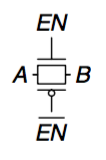
\includegraphics[width=0.15\textwidth]{pictures/transmissionGate.png}
  \end{wrapfigure}
  At times, designers find it convenient to use an ideal switch that can pass both 0 and 1 well. \\
  nMOS transistors are good at passing 0 and pMOS transistors are good at passing 1, so the parallel combination of the two passes both values well. \\
  Image to the right shows such a circuit, called \emph{transmission gate \emph{or} pass gate}. \\
  The two sides of the switch are called \emph{A \emph{and} B} because a switch is bidirectional and has no preferred input or output side.
  The control signals are called \emph{enables}, $EN$ and $\overline{EN}$. \\
  When $EN = 0$ and $\overline{EN} = 1$, both transistors are OFF.
  Hence, the transmission gate is OFF or disabled, so A and B are not connected. \\
  When $EN = 1$ and $\overline{EN} = 0$, the transmission is ON or enabled, and any logic value can flow between A and B.

  \subsection{Pseudo-nMOS Logic}
  An \emph{N}-input CMOS NOR gate uses \emph{N} nMOS transistors in parallel and \emph{N} pMOS transistors in series.
  Transistors in series are slower than transistors in parallel, just as resistors in series have more resistance than resistors in parallel. \\
  Moreover, pMOS transistors are slower than nMOS transistors because holes cannot move around the silicon lattice as fast as electrons.
  Therefore parallel nMOS transistors are fast and the series pMOS transistors are slow, especially when many are in series. \\

  Pseudo-nMOS logic replaces the slow stack of pMOS transistors with a single weak pMOS transistor that is always ON.
  This pMOS transistors is often called a \emph{weak pull-up}.
  The physical dimensions of the pMOS transistor are selected so that the pMOS transistor will pull the output, $Y$, HIGH weakly---that is, only if none of the nMOS transistors are ON.
  But if any nMOS transistor is ON, it overpowers the weak pull-up and pulls Y down close enough to GND to produce a logic 0. \\

  The advantage of pseudo-nMOS logic is that it can be used to build fast NOR gates with many inputs. \\
  The disadvantage is that a short circuit exists between $V_{DD}$ and GND when the output is LOW; the weak pMOS and nMOS transistors are both ON.
  The short circuit draws continuous power, so pseudo-nMOS logic must be used sparingly.

  \section{Summary So Far}
  \emph{There are 10 kinds of people in this world: those who can count in
binary and those who can't.} \\
  The real world is analog, though digital designers discipline themselves to use a discrete subset of possible signals.
  In particular, binary variables have just two states: 0 and 1, also called FALSE and TRUE or LOW and HIGH. \\

  Logic gates compute a binary output from one or more binary inputs.
  Some of the common logic gates are:
  \begin{itemize}
    \item[\textbf{NOT}:] TRUE when all input is FALSE
    \item[\textbf{AND}:] TRUE when all input are TRUE
    \item[\textbf{OR}:]  TRUE when any inputs are TRUE
    \item[\textbf{XOR}:] TRUE when an odd number of inputs are TRUE
  \end{itemize}

  Logic gates are commonly built from CMOS transistors, which behave as electrically controlled switches. \\
  nMOS transistors turn ON when the gate is 1. \\
  pMOS transistors turn ON when the gate is 0.

  \section{Introduction to Combinational Logic Design}
  In digital electronics, a \emph{circuit} is a network that processes discrete-valued variables. \\
  A circuit can be viewed as a black box, with
  \begin{itemize}
    \item one or more discrete-valued \emph{input terminals}
    \item one or more discrete-valued \emph{output terminals}
    \item a \emph{functional specification} describing the relationship between inputs and outputs
    \item a \emph{timing specification} describing the delay between inputs changing and output responding
  \end{itemize}
  Peering inside the black box, circuits are composed of nodes and elements. \\
  An \emph{element} is itself a circuit with inputs, outputs, and a specification. \\
  A \emph{node} is a wire, whose voltage conveys a discrete-valued variable.
  Nodes are classified as \emph{input, output, \emph{or} internal}. \\
  Input receive values from the external world. \\
  Output deliver values to the external world. \\
  Wires that are not inputs or outputs are called internal nodes. \\

  Digital circuits are classified as \emph{combinational \emph{or} sequential}. \\
  A combinational circuit's outputs depend only on the current values of the inputs; in other words, it combines the current input values to compute the output.
  For example, a logic gate is a combinational circuit. \\
  A sequential circuit's outputs depend on both current and previous values of the inputs; in other words, it depends on the input sequence. \\
  A combinational circuit is \emph{memoryless}, but a sequential circuit has \emph{memory}. \\

  The functional specification of a combination circuit expresses the output values in terms of the current input values. \\
  The timing specification of a combinational circuit consists of lower and upper bounds on the delay from input to put. \\

  To simply drawings, a single line with a slash through it and a number next to it is often used to indicate a \emph{bus}, a bundle of of multiple signals.
\\
  \begin{wrapfigure}{l}{0.25\textwidth}
    \centering
    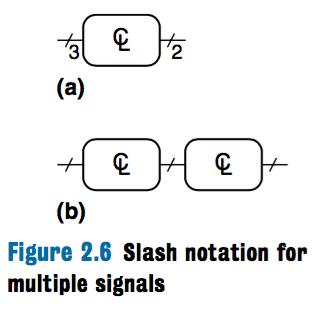
\includegraphics[width=0.25\textwidth]{pictures/busExample.png}
  \end{wrapfigure}
  In Figure 2.6(a), it represents a block of combination logic with three inputs and output outputs. \\
  If the number of bits is unimportant or obvious from the context, the slash may be shown without a number. \\
  Figure 2.6(b) indicates two blocks of combinational logic with an arbitrary number of outputs from one block serving as inputs to the second block. \\

  The rules of \emph{combinational composition} tell us how we can build a large combinational circuit from smaller combinational circuit elements. \\
  A circuit is combinational if it consists of interconnected circuit elements such that:
  \begin{itemize}
    \item Every circuit element is itself combinational
    \item Every node of the circuit is either designated as an input to the circuit or connects to exactly one output terminal of a circuit element
    \item The circuit contains no cyclic paths: every path through the circuit visits each circuit node at most once
  \end{itemize}

  Examples: \\
  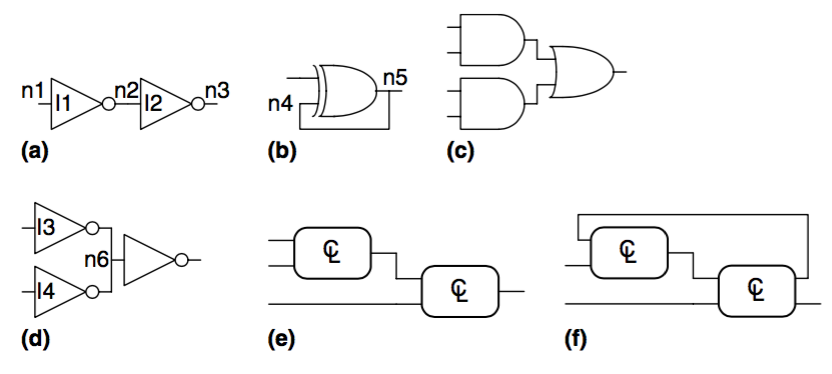
\includegraphics{pictures/combinationalCircuitExample.png}
  (a) is combinational. It is constructed from two combinational circuit elements (inverters $I1$ and $I2$). It has three nodes: $n1$, $n2$, and $n3$. $n1$ is an input to the circuit and to $I1$; $n2$ is an internal node, which is the output of $I1$ and the input to $I2$; $n3$ is the output of the circuit and of $I2$. \\
  (b) is \emph{not} combinational, because there is a cyclic path: the output of the XOR feeds back to one of its input. Hence, a cyclic path starting at $n4$ passes through the XOR to $n5$, which returns to $n4$. \\
  (c) is combinational. \\
  (d) is not combinational, because node $n6$ connects to the output terminals of both $I3$ and $I4$. \\
  (e) is combinational, illustrating two combinational circuits connecting to from a larger combinational circuit. \\
  (f) does not obey the rules of combinational composition because it has a cyclic path through the two elements. Depending on the functions of the elements, it may or may not be a combinational circuit. \\

  The functional specification of a combinational circuit is usually expressed as a truth table or a Boolean equation.

  \section{Boolean Equations}
  Boolean equations deal with variables that are either TRUE or FALSE, so they are perfect for describing digital logic.

  \subsection{Terminology}
  The \emph{complement} of a variable, $A$, is its inverse, $\overline{A}$. \\
  The variables or its complement is called a \emph{literal}.
  For example, $A$, $\overline{A}$, $B$, and $\overline{B}$ are literals. \\
  $A$ is called the \emph{true form} of the variable and $\overline{A}$ the complementary form; ``true form'' does not mean that $A$ is TRUE, but merely that $A$ does not have a line over it. \\

  The AND of one or more literals is called a \emph{product} or an \emph{implicant}. \\
  $\overline{A}B$, $A\overline{B} \overline{C}$, and $B$ are all implicants for a function of three variables. \\
  A \emph{minterm} is a product involving all of the inputs to the function.
  $A\overline{B}\overline{C}$ is a minterm for a function of the three variables $A$, $B$, and $C$, but $\overline{A}B$ is not, because it does not involve $C$. \\

  Similarly, the OR of one or more literals is called a \emph{sum}.
  A \emph{maxterm} is a sum involving all of the inputs to the function. $A + \overline{B} + C$ is a maxterm for a function of the three variables $A$, $B$, and $C$.

  \subsection{Sum-of-Products Form}
  A truth table of $N$ inputs contains $2^{N}$ rows, one for each possible value of the inputs. \\
  Each row in a truth value is associated with a minterm that is TRUE for that row. \\
  A Boolean equation can be written for any truth table by summing each of the minterms for which the output, $Y$, is TRUE.
  This is called the \emph{sum-of-products canonical form} of a function because it is the sum (OR) of products (ANDs forming minterms). \\

  The sum-of-products form provides a Boolean equation for any truth table with any number of variables.
  Unfortunately, it does not necessarily generate the simplest equation.

  \section{Boolean Algebra}
  \subsection{Axioms}
  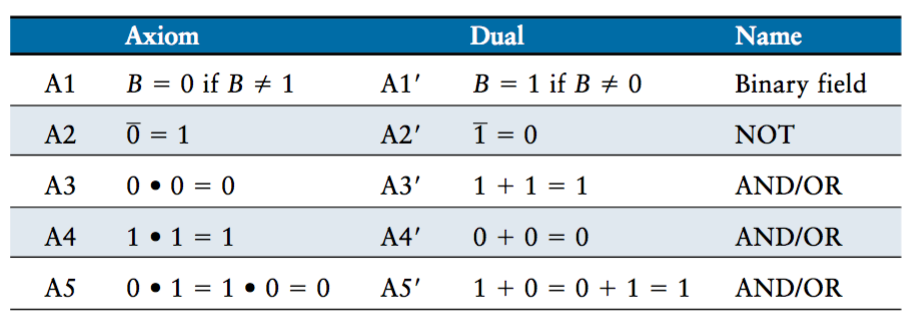
\includegraphics[scale=0.7]{pictures/booleanAlgAxiom.png}

  \subsection{Theorems of One Variable}
  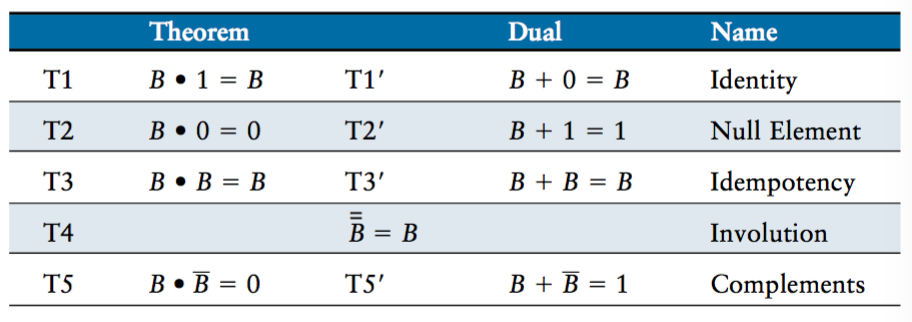
\includegraphics[scale=0.7]{pictures/booleanAlgOneVari.png}

  \subsection{Theorems of Several Variables}
  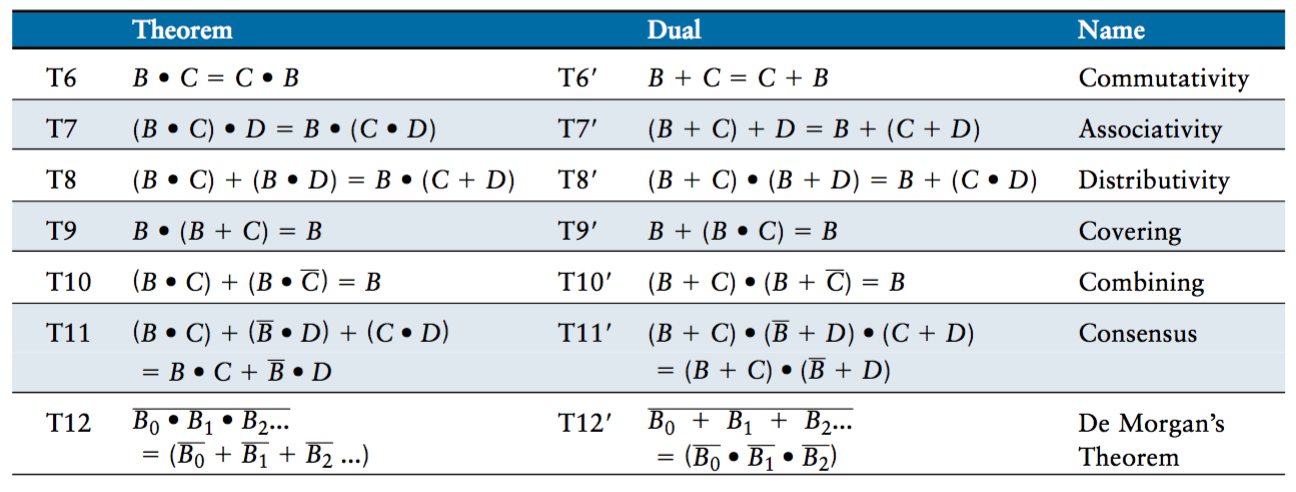
\includegraphics[scale=0.65]{pictures/booleanAlgMultVar.png}

  \section{From Logic to Gates}
  A \emph{schematic} is a diagram of a digital circuit showing the elements and the wires that connect them together. \\

  \textbf{Good Style in Circuit Drawing}:
  \begin{itemize}
    \item Assume all literals (variables and their negations) are available
    \item Rectilinear wires, dots when wires split
    \item Do not draw spaghetti wires for inputs; instead, write each literal as needed
  \end{itemize}

  \section{Multilevel Combinational Logic}
  Logic in sum-of-products form is called \emph{two-level logic} because it consists of literals connected to a level of AND gates connected to a level of OR gates. \\
  Designers often build circuits with more than two levels of logic gates.
  These multilevel combinational circuits may use less hardware than their two-level counterparts. \\
  Bubble pushing is especially helpful in analyzing and designing multilevel circuits.

  \subsection{Hardware Reduction}
  Some logic functions require an enormous amount of hardware when built using two-level logic.
  A notable example is the XOR function of multiple variables. \\
  A three-input XOR can be built out of a cascade of two-input XORs. \\
  Similarly, an eight-input XOR would require 128 eight-input AND gates and one 128-input OR gate for a two level-sum-of-products implementation. A much better option is to use a tree of two-input XOR gates. \\

  ``Best'' has many meanings: fewest gates, fastest, shortest design time, least cost, least power consumption. \\
  ``Best'' circuit in one technology is not necessarily the best in another.
  ANDs and ORs are used often, but in CMOS, NANDs and NORs are more efficient.

  \subsection{Bubble Pushing}
  CMOS circuits prefer NANDs and NORs over ANDs and ORs.
  However, reading the equation by inspection can be difficult. \\
  Bubble pushing is a helpful way to redraw these circuits so that the bubbles cancel out and the function can be more easily determined. \\
  Guidelines for bubble pushing:
  \begin{itemize}
    \item Begin at the output of the circuit and work toward the inputs.
    \item Push any bubbles on the final output back toward the inputs so that you can read an equation in terms of the output.
    \item Working backward, draw each gate in a form so that bubbles cancel. If the current gate has an input bubble, draw the preceding gate with an output bubble. If the current gate does not have an input bubble, draw the preceding gate without an output bubble.
  \end{itemize}

  \section{Combinational Building Blocks}
  Combinational logic is often grouped into larger building blocks to build more complex systems.
  This is an application of the principle of abstraction, hiding the unnecessary gate-level details to emphasize the function of the building block.

  \subsection{Multiplexers}
  \emph{Multiplexers}, also known as \emph{mux}, are among the most commonly used combinational circuits.
  They choose an output from among several possible inputs based on the value of a \emph{select} signal.

  \subsubsection{2:1 Multiplexer}
  \begin{wrapfigure}{r}{0.25\textwidth}
    \centering
    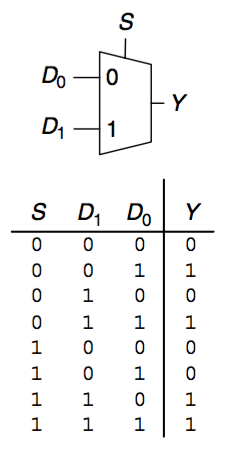
\includegraphics[width=0.25\textwidth]{pictures/2_1_mux.png}
  \end{wrapfigure}
  Image shows the schematic and truth table for a 2:1 multiplexer with two data inputs, $D_0$ and $D_1$, as select input, $S$, and one output, $Y$. \\
  The multiplexer chooses between the two data inputs based on the select:
  if $S = 0$, $Y = D_0$, and if $S = 1$, $Y = D_1$.  \\
  $S$ is also called a control signal because it controls what the multiplexer does. \\

  Multiplexers can be built from tristate buffers. \\
  The tristate enables are arranged such that, at all times, exactly one tristate buffer is active. \\
  When $S = 0$, tristate $T_0$ is enabled, allowing $D_0$ to flow to $Y$. \\
  When $S = 1$, tristate $T_1$ is enabled, allowing $D_1$ to flow to $Y$.

  \subsubsection{Wider Multiplexers}
  A 4:1 multiplexer has four data inputs and one output.
  Two select signals are needed to choose among the four data inputs.
  The 4:1 mux can be built using sum-of-products logic, tristates, or multiple 2:1 mux. \\

  The product terms enabling the tristates can be formed using AND gates and inverters.
  They can also be formed using a decoder. \\

  In general, an $N:1$ multiplexer needs $log_{2} N$ select lines.

  \subsubsection{Multiplexer Logic}
  Multiplexers can be used as \emph{lookup tables} to perform logic functions.
 \\
  In general, a $2^{N}$-input multiplexer can be programmed to perform any N-input logic functions by applying 0's and 1's to the appropriate data inputs. \\
  By changing the data inputs, the multiplexer can be reprogrammed to perform a different function.

  \subsection{Decoder}
  A decoder has $N$ inputs and $2^{N}$ outputs. \\
  It asserts exactly one of its outputs depending on the input combination.
  The outputs are called \emph{one-hot}, because exactly one is ``hot'' (HIGH) at a given time. \\

  Example of 2:4 decoder and its implementation: \\
  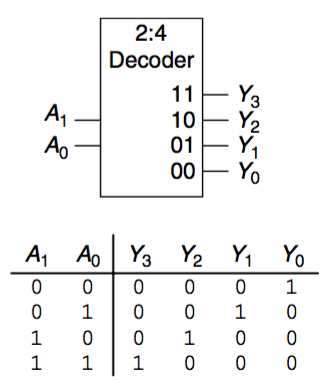
\includegraphics{pictures/2_4_decoder.png}
  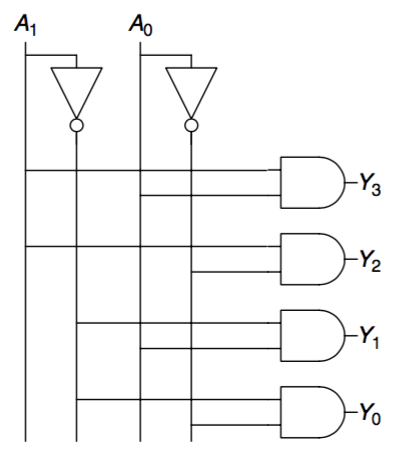
\includegraphics{pictures/2_4_decoder_implementation.png} \\

  \subsubsection{Decoder Logic}
  Decoders can be combined with OR gates to build logic functions. \\
  When using decoders to build logic, it is easiest to express functions as a truth table or in canonical sum-of-products form.
  A $N$-input function with $M$ 1's in the truth table can be built with an $N:2^{N}$ decoder and an $M$-input or gate attached to all of the minterms containing 1's in the truth table.

  \section{Summary So Far}
  A digital circuit is a module with discrete-valued inputs and outputs and a specification describing the function and timing of the module. \\

  The function of a combinational circuit can be given by a truth table or a Boolean equation. The Boolean equation for any truth table can be obtained systematically using sum-of-products or product-of-sums form. \\
  In sum-of-products form, the function is written as the sum (OR) of one or more implicants.
  Implicants are the product (AND) of literals.
  Literals are the true or complementary forms of the input variables.  \\

  Boolean equation can be simplified using the rules of Boolean algebra.
  In particular, they can be simplified into minimal sum-of-products form by combining implicants that differ only in the true and complementary forms of one of the literals: $PA + P\overline{A} = P$. \\

  Logic gates are connected to create combinational circuits that perform the desired function. \\
  Any functions in sum-of-products form can be built using two-level logic with the literals as inputs: NOT gates form the complementary literals, AND gates form the products, and OR gates form the sum. \\
  CMOS circuits favor NAND and NOR gates because these gates can be built directly from CMOS transistors without requiring extra NOT gates. \\
  When using NAND and NOR gates, bubble pushing is helpful to keep track of the inversions. \\

  Logic gates are combined to produce larger circuits such as multiplexers, decoders, and priority circuits. \\
  A multiplexer chooses one of the data inputs based on the select input. \\
  A decoder sets one of the outputs HIGH according to the input. \\
  A priority circuit produces an output indicating the highest priority input. \\

  The timing specification of a combinational circuit consists of the propagation and contamination delays through the circuit. \\
  These indicate the longest and shortest times between an input change and the consequent output change. \\
  Calculating the propagation delay of a circuit involves identifying the critical path through the circuit, then adding up the propagation delays of each element along that path.

  \section{Introduction to Sequential Logic Design}
  The output of sequential logic depend on both current and prior input values. \\
  Hence, sequential logic has memory.
  Sequential logic might explicitly remember certain previous inputs, or it might distill the prior inputs into a smaller amount of information called the \emph {state} of the system. \\
  The state of a digital sequential circuit is a set of bits called \emph{state variables} that contain all the information about the past necessary to explain the future behavior of the circuit.

  \section{Latches and Flip-Flops}
  The fundamental building block of memory is a \emph{bistable} element, an element with two stable states. \\
  An element with $N$ stable states conveys $\log_{2}N$ bits of information, so a bistable element stores one bit. \\
  The state of the cross-coupled inverters is contained in one binary state variable, $Q$.
  The value of $Q$ tells us everything about the past that is necessary to explain the future behavior of the circuit. \\
  Specifically, if $Q = 0$, it will remain 0 forever, and if $Q = 1$, it will remain 1 forever. \\
  The circuit does have another node, $\overline{Q}$, but $\overline{Q}$ does not contain any additional information because if $Q$ is known, $\overline{Q}$ is also known.
  $\overline{Q}$ is also an acceptable choice for the state variable. \\

  When power is first applied to a sequential circuit, the initial state is unknown and usually unpredictable.
  It may differ each time the circuit is turned on. \\

  Although the cross-coupled inverters can store a bit of information, they are not practical because the user has no inputs to control the states. \\
  However, other bistable elements, such as \emph{latches} and \emph{flip-flops}, provide inputs to control the value of the state variable.

  \blfootnote{Just a $Y$ is commonly used for the output of combinational logic, $Q$ is commonly used for the output of sequential logic.}

  \newpage

  \subsection{SR Latch}
  \begin{wrapfigure}{r}{0.25\textwidth}
    \centering
    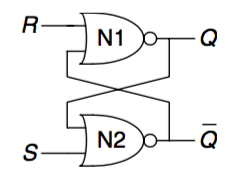
\includegraphics[width=0.25\textwidth]{pictures/srLatch.png}
  \end{wrapfigure}

  \emph{SR latch} is one of the simplest sequential circuit as it is composed of two cross-coupled NOR gates. \\
  The latch has two inputs, $S$ and $R$, and two outputs, $Q$ and $\overline{Q}$. \\
  The SR latch is similar to the cross-coupled inverters, but its state can be controlled through the $S$ and $R$ inputs, which \emph{set} and \emph{reset} the output $Q$. \\

  Consider the four possible combinations of $R$ and $S$:
  \begin{itemize}
    \item[\emph{Case I:}] $R = 1, S = 0$ \\
    N1 sees at least one TRUE input, $R$, so it produces a FALSE output on $Q$. N2 sees both $Q$ and $S$ FALSE, so it produces a TRUE output on $\overline{Q}$.
    \item[\emph{Case II:}] $R = 0, S = 1$ \\
    N1 receives inputs of 0 and $\overline{Q}$. Because we don't yet know $\overline{Q}$, we can't determine the output $Q$. N2 receives at least one TRUE input, $S$, so it produces a FALSE output on $\overline{Q}$. Now we can revisit N1, knowing that both inputs are FALSE, so the output $Q$ is TRUE.
    \item[\emph{Case III:}] $R = 1, S = 1$ \\
    N1 and N2 both set at least one TRUE input ($R$ or $S$), so each produces a FALSE output. Hence $Q$ and $\overline{Q}$ are both FALSE.
    \item[\emph{Case IV:}] $R = 0, S = 0$ \\
    N1 receives inputs of 0 and $\overline{Q}$. Because we don't yet know $\overline{Q}$, we can't determine the output. N2 receives inputs of 0 and $Q$. Because we don't yet know $Q$, we can't determine the output. Now we are stuck. This is reminiscent of the cross-coupled inverters. But we know that $Q$ must either be 0 or 1. So we can solve the problem by checking what happens in each of these sub-cases.
    \item[\emph{Case IVa:}] $Q = 0$ \\
    Because $S$ and $Q$ are FALSE, N2 produces a TRUE output on $\overline{Q}$. Now N1 receives one TRUE input, $\overline{Q}$, so its output, $Q$, is FALSE.
    \item[\emph{Case IVb:}] $Q = 1$ \\
    Because $Q$ is TRUE, N2 produces a FALSE output on $\overline{Q}$. Now N1 receives two FALSE inputs, $R$ and $\overline{Q}$, so its output, $Q$, is TRUE.
  \end{itemize}

  Suppose $Q$ has some known prior value, $Q_{prev}$, before we enter Case IV. $Q_{prev}$ is either 0 or 1, and represents the state of the system.
  When $R$ and $S$ are 0, $Q$ will remember this old value, $Q_{prev}$, and $\overline{Q}$ will be its complement, $\overline{Q}_{prev}$.
  This circuit has memory. \\

  Like the cross-coupled inverters, the SR latch is a bistable element with one bit of state stored in $Q$.
  However, the state can be controlled through the $S$ and $R$ inputs. \\
  When $R$ is asserted, the state is reset to 0. \\
  When $S$ is asserted, the state is set to 1. \\
  When neither is asserted, the state retains its old value.

  \subsection{D Latch}
  The SR latch is awkward because it behaves strangely when both $S$ and $R$ are simultaneously asserted.
  Moreover, the $S$ and $R$ inputs conflate the issues of \emph{what} and \emph{when}.
  Asserting one of the inputs determines not only \emph{what} the state should be but also \emph{when} it should change. \\
  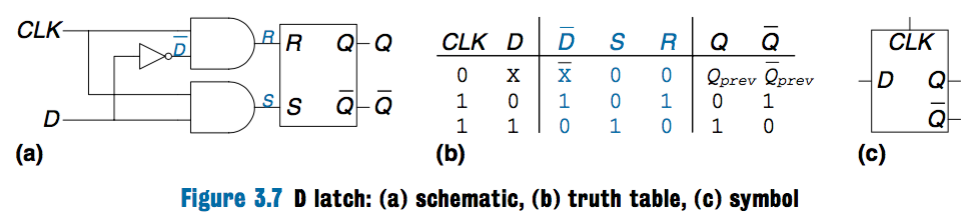
\includegraphics[width=1.0\textwidth]{pictures/dLatch.png}\\
  The D latch has two inputs.
  The \emph{data} input, $D$, controls what the next state should be.
  The \emph{clock} input, $CLK$, controls when the state should change. \\
  The clock controls when data flows through the latch. \\
  When $CLK = 1$, the latch is \emph{transparent}.
  The data at $D$ flows through to $Q$ as if the latch were just a buffer. \\
  When $CLK = 0$, the latch is \emph{opaque}.
  It blocks the new data from flowing through to $Q$, and $Q$ retains the old value. \\
  The D latch updates its state continuously $CLK = 1$.
  \newpage
  \subsection{D Flip-Flop}
  \begin{wrapfigure}{r}{0.3\textwidth}
    \centering
    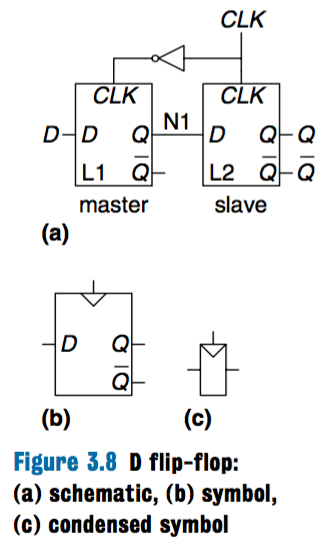
\includegraphics[width=0.3\textwidth]{pictures/dFlipFlop.png}
  \end{wrapfigure}
  A \emph{D flip-flop} can be built from two back-to-back D latches controlled by complementary clocks. \\
  The first latch, $L1$, is called the \emph{master}. \\
  The second latch, $L2$, is called the \emph{slave}. \\
  The node between them is named $N1$. \\
  A symbol for the D flip-flop is given in the figure (b). \\
  When the $\overline{Q}$ output is not needed, the symbol can be condensed as in figure (c). \\

  When $CLK = 0$, the master latch is transparent and the slave is opaque.
  The value at $D$ propagates through to $N1$. \\
  When $CLK = 1$, the master goes opaque and the slave becomes transparent.
  The value at $N1$ propagates through to $Q$, but $N1$ is cut off from $D$.
  Hence, the value at $D$ immediately before the clock rises from 0 too 1 gets copied to $Q$ immediately after the clock rises. \\
  At other times, $Q$ retains its old value, because there is always an opaque latch blocking the path between $D$ and $Q$.

  \begin{figure}[!ht]
  \centering
  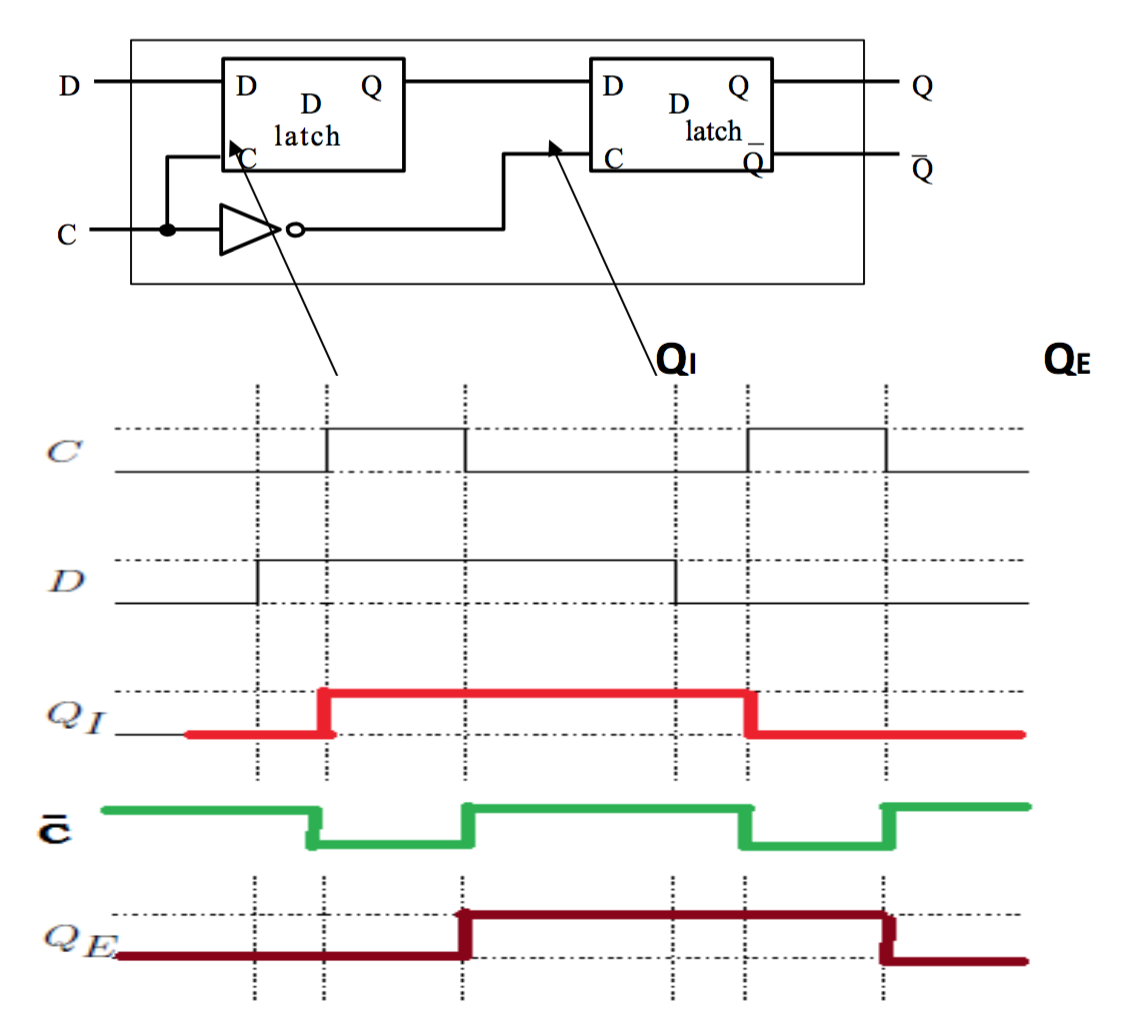
\includegraphics[width=0.55\textwidth]{pictures/dFlipFlopExample.png} \\
  \caption{A D flip-flop example.}
  \end{figure}
  A \emph{D flip-flop} copies $D$ to $Q$ on the rising edge of the clock, and remembers its state at all other times. \\

  A D flip-flop is also known as a \emph{master-slave flip-flop}, an \emph{edge-triggered flip-flop}, or a \emph{positive edge-triggered flip-flop}.

  \subsection{Register}
  A $N$-bit register is a bank of $N$ flip-flops that share a common $CLK$ input, so that all bits of the register are updated at the same time. \\
  Registers are the key building block of most sequential circuits. \\

  For a 32-bit architectures, a register would typically have 32 flip-flops in parallel (i.e. one for each bit). \\
  A \emph{register file} is a way of organizing registers. \\
  \includePicture{1.0}{pictures/registerFile.png}{A register file.} \label{registerFile}

  \subsubsection{Reading from a Register File}
  The values of all 32 registers go through two multiplexers. \\
  The first multiplexer determines which register value will be routed to the 1\textsuperscript{st} output. \\
  The second multiplexer determines which register value will be routed to the 2\textsuperscript{nd} output. \\
  It will take 5 select lines to uniquely identify each source register (when there are 32 registers).

  \subsubsection{Writing to a Register File}
  The address of the register $d$, is routed through a decoder which determines which D flip-flop to write to. \\
  When the $d^{\text{th}}$ decoder line and the \emph{RegWrite} line are both 1, they pass a 1 through the $d^{\text{th}}$ AND gate and raise the $C$ input of the $d^{\text{th}}$ D flip-flop to 1. \\
  The data will now be written to Register $\$d^{\text{th}}$.

  \section{Finite State Machines}
  Synchronous sequential circuits can be drawn in the forms called \emph{finite state machines (FSMs)}.
  The name comes from a circuit with $k$ registers can be in one of a finite number ($2^{k}$) of unique states. \\
  A FSM has $M$ inputs, $N$ outputs, and $k$ bits of state.
  It also receives a clock and, optionally, a reset signal. \\
  An FSM consists of two blocks of combinational logic, \emph{next state logic} and \emph{output logic}, and a register that stores the state.
  On each clock edge, the FSM advances to the next state, which was computed based on the current state and inputs. \\
  Finite state machines provides a systematic way to design synchronous sequential circuits given a functional specification.

  Two general classes of finite state machines, characterized by their functional specifications. \\
  In \emph{Moore machines}, the outputs depend only on the current state of the machine. \\
  In \emph{Mealy machines}, the outputs depend on both the current state and the current inputs.

  \begin{wrapfigure}{r}{0.4\textwidth}
    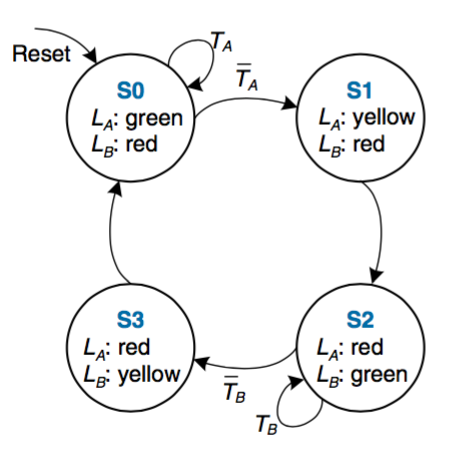
\includegraphics[width=0.4\textwidth]{pictures/stateTransistionDiagram.png}
  \end{wrapfigure}

  \subsection{State Transition Diagram}
  A \emph{state transition diagram} indicates all the possible states of the system and the transitions between these states. \\
  In a state transition diagram, circles represent states and arcs represent transitions betweens states. \\
  The transitions take place on the rising edge of the clock; the clock can hidden on the diagram because it is always present in a synchronous sequential circuit.
  In addition, the clock only controls when the transitions should occur, whereas the diagram indicates which transitions occur. \\
  If a state has multiple arcs leaving it, the arcs are labeled to show what input triggers each transition.
  In the image, when in state $S0$, the system will remain in that state if $T_{A}$ is TRUE and move to $S1$ if $T_{A}$ is FALSE. \\
  If a state has a single arc leaving it, that transition always occurs regardless of the inputs.
  In the image, when in state $S1$, the system will always move to $S2$. \\

  \subsection{State Transition Table}
  \includePicture{0.8}{pictures/stateTTableStateEncode.png}{Example Transition Table and its Encoding}
  A \emph{state transition table} indicates for each state and input, what the next state, $S'$, should be.
  If the next state does not depend on a particular input, the don't care symbol (X) is used. \\
  To build a real circuit, the states and outputs must be assigned \emph{binary encodings}.

  \subsection{State Encoding}
  If the state and output encodings were selected arbitrarily, a different choice would have resulted in a different circuit. \\
  Then how to determine the encoding that produces the circuit with the fewest logic gates or the shortest propagation delay?
  There is not simply method to find the best encoding. \\
  It is possible to choose a good encoding by inspection, so that related states share bits. \\

  An important decision in state encoding is the choice between binary encoding and one-hot encoding. \\
  With \emph{binary encoding}, each state is represented as a binary number.
  Because $K$ binary numbers can be represented by $\log_{2}K$ bits, a system with $K$ states only needs $\log_{2}K$ bits of state. \\

  In \emph{one-hot encoding},  a separate bit of state is used for each state.
  It is called one-hot because only one bit is ``hot'' or TRUE at any time.
  \begin{ex}
    A one-hot encoded FSM with three states would have state encodings of 001, 010, and 100.
  \end{ex}
  Each bit of state is stored in a flip-flop, so one-hot encoding requires more flip-flops than binary encoding.
  However, with one-hot encoding, the next-state and output logic is often simpler, so fewer gates are required. \\

  Another encoding is the \emph{one-cold} encoding, in which $K$ states are represented with $K$ bits, exactly one of which is FALSE.

  \subsection{FSM Review} \label{FSM_Review}
  Finite state machines are a powerful way to systematically design sequential circuits from a written specification. \\
  Procedure to design an FSM:
  \begin{enumerate}
    \item[>] Identify the inputs and outputs.
    \item[>] Sketch a state transition diagram.
    \item[>] For a Moore machine:
    \begin{enumerate}
      \item[-] Write a state transition table.
      \item[-] Write an output table.
    \end{enumerate}
    \item[>] For a Mealy machine:
    \begin{enumerate}
      \item[-] Write a combined state transition and output table.
    \end{enumerate}
    \item[>] Select state encodings---selection affects the hardware design.
    \item[>] Write Boolean equations for the next state and output logic.
    \item[>] Sketch the circuit schematics.
  \end{enumerate}

  \section{Summary So Far}
  In contrast to combinational logic, whose outputs depend solely on the current inputs, sequential logic outputs depend on both current and prior inputs.
  Sequential logic remembers information about prior inputs.
  This memory is called the state of the logic. \\

  Sequential circuits can be difficult to analyze and are easy to design incorrectly.
  An important element is the flip-flop, which receives a clock and an input, $D$, and produces an output, $Q$.
  The flip-flop copies $D$ to $Q$ on the rising edge of the clock and otherwise remembers the old state of $Q$.
  A group of flip-flops sharing a common clock is called a register.
  Flip-flops may also receive reset or enable control signals. \\

  Finite state machines are a powerful technique for designing sequential circuits.
  For procedure on designing an FSM, refer to \ref{FSM_Review} (FSM Review). \\

  Synchronous sequential circuits have a timing specification including to clock-to-$Q$ propagation and contamination delay, $t_{pcq}$ and $t_{ccq}$, and the setup and hold times, $t_{setup}$ and $t_{hold}$. \\
  For correct operation, their inputs must be stable during an aperture time that starts a setup time before the rising edge of the clock and ends a hold time after the rising edge of the clock. \\

  The minimum cycle time, $T_{c}$, of the system is equal to the propagation delay, $t_{pd}$, through combinational logic plus $t_{pcq} + t_{setup}$ of the register. \\
  For correct operation, the contamination delay through the register and combinational logic must be greater than $t_{hold}$.
  Hold time does not affect the cycle time. \\

  Overall performance is measured in latency and throughput.
  The latency is the time required for a token to pass from start to end.
  The throughput is the number of tokens that the system can process per unit time.
  Parallelism improves the system throughput.

  \section{Multiplication}
  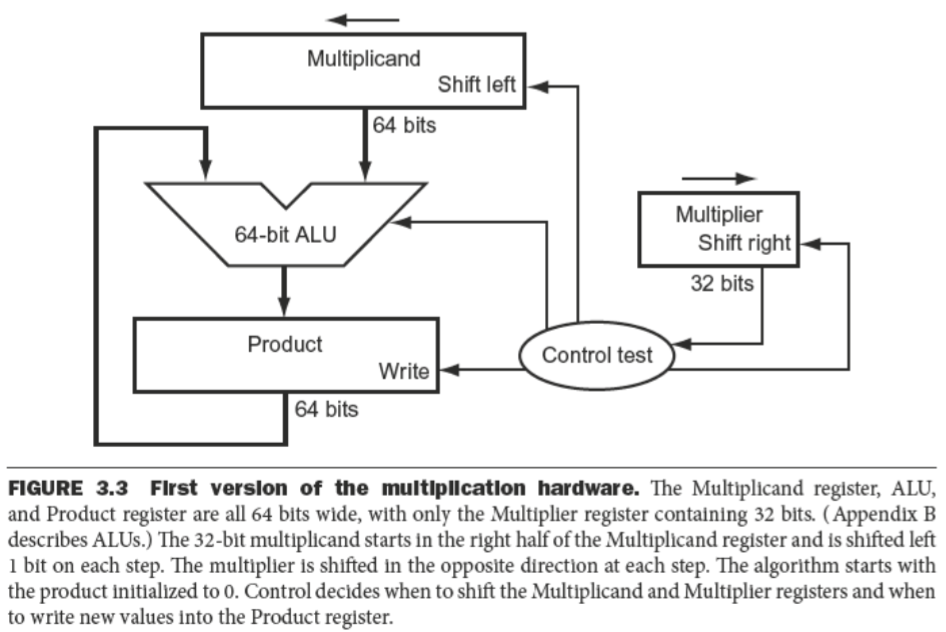
\includegraphics[width=1.0\textwidth]{pictures/multiplication.png} \\
  The first operand is called the \emph{multiplicand} and the second the \emph{multiplier}.
  The final result is called the \emph{product}. \\\
  Number of bits in the product is considerably larger than the number in either the multiplicand or the multiplier.
  If ignoring the sign bit, the length of the multiplication of an $n$-bit multiplicand and an $m$-bit multiplier is a product that is $n + m$ bits long.
  So $n + m$ bits are required to represent all possible products.

  \section{Floating Point}
  A number in scientific notation that has no leading 0s is called a \emph{normalized} number, which is the usual way to write it. \\
  \emph{Floating point} is computer arithmetic that represents numbers in which the binary point is not fixed. \\
  A standard scientific notation for reals in normalized form offers tree advantages:
  \begin{enumerate}
    \item It simplifies exchange of data that includes floating-point numbers.
    \item It simplifies the floating-point arithmetic algorithms to know that numbers will always be in this form.
    \item It increases the accuracy of the numbers that can be stored in a word, since the unnecessary leading 0s are replaced by real digits to the right of the binary point.
  \end{enumerate}

  \subsection{Floating-Point Representation}
  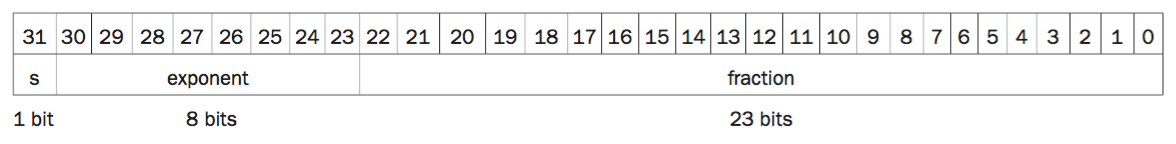
\includegraphics[width=1.0\textwidth]{pictures/mipsFloat.png} \\
  $s$ is the sign of the floating-point number (1 meaning negative).
  \emph{exponent} is the value of the 8-bit exponent field (including the sign of the exponent).
  \emph{fraction} is the 23-bit number. \\
  Generally, floating-point numbers are of the form: $$(-1)^{s} \times F \times 2^{E}$$
  F involves the value in the fraction field and E involves the value in the exponent field.

  \blfootnote{\emph{overflow}: positive exponent becomes too large to fit in the exponent field}
  \blfootnote{\emph{underflow}: negative exponent becomes too large to fit in the exponent field}

  A \emph{double precision} floating-point number is represented in two 32-bit words.
  The exponent is the value of the 11-bit exponent field.
  Fraction is the 52-bit number in the fraction field. \\
  \includePicture{0.85}{pictures/floatingPoints.png}{IEEE 754 encoding of floating-point numbers.}

  This is also known as the \emph{IEEE 754 floating-point standard}.
  This standard has greatly improved both the ease of porting floating-point programs and the quality of computer arithmetic. \\
  In IEEE 754, the leading 1-bit of normalized binary number is implicit, so the number is actually 24 bits long in single precision. \\

  For the fractional part, suppose we number the bits of the fraction from left to right $s1$, $s2$, $s3$, \dots, then the value is
  $$(-1)^{S} \times (1 + (s1 \times 2^{-1}) + (s2 \times 2^{-2}) + (s3 \times 2^{-3}) + (s4 \times 2^{-4}) + \dots) \times 2^{E}$$

  IEEE 754 uses a bias of 127 for single precision exponent. \\
  The exponent bias for double precision is 1023. \\
  So the value represented by a floating-point number is really
  $$(-1)^{S} \times (1 + \text{Fraction}) \times 2^{(\text{Exponent} - \text{Bias})}$$

  \subsection{Floating-Point Addition}
  \begin{itemize}
    \item[1.] Compare the exponents of the two numbers; shift the smaller number to the right until its exponent would match the larger exponent.
    \item[2.] Add the significants.
    \item[3.] Normalize the sum, either shifting right and incrementing the exponent or shifting left and decrementing the exponent.
    \item[>] Overflow or underflow? If yes, Exception. Otherwise, continue.
    \item[4.] Round the significant to the appropriate number of bits.
    \item[>] Still normalized? If no, then step 3. Otherwise, done.
  \end{itemize}
  \includePicture{0.7}{pictures/floatingAddition.png}{Arithmetic unit for floating-point addition.}

  \subsection{Floating-Point Multiplication}
  \begin{itemize}
    \item[1.] Add the biased exponents of the two numbers, subtracting the bias from the sum to get the new biased exponent.
    \item[2.] Multiply the significants.
    \item[3.] Normalize the product if necessary, shifting it right and incrementing the exponent.
    \item[>] Overflow or underflow? If yes, Exception. Otherwise, continue.
    \item[4.] Round the significant to the appropriate number of bits.
    \item[>] Still normalized? If no, then Step 3. Otherwise, continue.
    \item[5.] Set the sign of the product to positive if the signs of the original operands are the same; if they differ, make the sign negative.
  \end{itemize}

  \section{Introduction to the Processor}
  A subset of the core MIPS instruction set will be examined:
  \begin{enumerate} \label{instruction_classes}
    \item[>] The memory-reference instructions \emph{load word} (lw) and \emph{store word} (sw)
    \item[>] The arithmetic-logical instructions add, sub, AND, OR, and slt
    \item[>] The branch instructions \emph{branch equal} (beq) and \emph{jump} (j)
  \end{enumerate}
  To implement those instructions, the first two steps are identical:
  \begin{enumerate}
    \item Send the \emph{program counter} (PC) to the memory that contains the code and fetch the instruction from that memory.
    \item Read one or two registers, using fields of the instruction to select the registers to read. For the load word instruction, only need to read one register, but most other instructions require reading two registers.
  \end{enumerate}
  After the two steps, the required actions depend on the instruction class.
  For each of the three instructions classes (\ref{instruction_classes}), the actions are largely the same, independent of the exact instruction. \\
  The simplicity and regularity of the MIPS instruction set simplifies the implementation by making the execution of many of the instruction classes similar. \\

  All instruction classes, except jump, use the arithmetic-logical unit (ALU) after reading the registers.
  The memory-reference instructions use the ALU for an address calculation, the arithmetic-logical instructions for the operation execution, and branches for comparison. \\
  After using the ALU, the actions required to complete various instruction classes differ. \\
  A memory-reference instruction will need to access the memory either to read data for a load or write data for a store. \\
  An arithmetic-logical or load instruction must write the data from the ALU or memory back into a register. \\
  For a branch instruction, it may be required to change the next instruction address based on the comparison; otherwise, the PC should be incremented by 4 to get the address of the next instruction.

  \section{Building a Data-path}
  \includePicture{0.7}{pictures/readingFetchingInstruction.png}{A portion of the data-path used for fetching instructions and incrementing the program counter.}
  A \emph{data-path element} is a unit used to operate within a processor.
  In the MIPS implementation, the data-path element include the instruction and data memories, the register file, the ALU, and adders. \\
  To execute any instruction, start by fetching the instruction from memory.
  Then increment the program counter so that it points at the next instruction, 4 bytes later. \\
  Refer to the figure above for how the elements are combined, forming a data-path that fetches instructions and increments the PC. \\

  A \emph{R-type \emph{or} R-format} is an arithmetical-logical instruction since they perform. \\
  All R-format instructions read two registers, perform an ALU operation on the contents of the register, and write the result to a register. \\

  Through a register file, it contains the register state of the computer and the ALU needs to operate on the values read from the registers. \\
  R-format instructions have three register operands, to read two data words from the register file and write one data word into the register file for each instruction. \\
  For each data word to be read from the register, an input to the register file is needed that will carry the value that has been read from the registers. \\
  To write a data word, two inputs are needed: one to specify the register number to be written and one to supply the \emph{data} to be written into the register. \\
  The register file always outputs the contents of whatever register numbers are on the Read register inputs.
  However, writes are controlled by the write control signal, which must be asserted for a write to occur at the clock edge. \\

  Thus, we need a total of four inputs (three for register number and one for data) and two outputs (both for data).
  The register number inputs are 5 bits wide to specify one of 32 registers ($32 = 2^{5}$), whereas the data input and two data output buses are each 32 bits wide (each word is 32 bits).

  \subsection{R-Format ALU Operations}
  Two elements are needed to implement R-format ALU operations: register file (\ref{registerFile}) and the ALU. \\

  The register file contains all the registers and has two read ports and one write port.
  The register file outputs the contents of the registers corresponding to the Read register inputs on the outputs; no other control inputs are needed. \\
  Note that a register write must be explicitly indicated by asserting the write control signal, $RegWrite$.
  Writes are edge-triggered, so that all write inputs must be valid at the clock edge. \\

  The inputs carrying the register number to the register file are all 5 bites wide, whereas the lines carrying data values are 32 bits wide. \\
  The operation to be performed by the ALU is controlled with the ALU operation signal, which will be 4 bits wide.

  \subsection{Memory-Reference Operations}
  \includePicture{0.75}{pictures/elementsFormemoryReference.png}{Two units needed for loads and stores. In addition to the register file and ALU.}
  Consider $lw$ and $sw$ instructions.
  They compute a memory address by adding the base register to the 16-bit signed offset field contained in the instruction. \\
  If the instruction is a store, the value to be stored must also be read from the register file where it resides in the destination register. \\
  If the instruction is a load, the value read from memory must be written into the register file in the specified register. \\
  Thus, both register and the ALU are required in addition to more. \\

  We need a unit to \emph{sign-extend} the 16-bit offset field in the instruction to a 32-bit signed value, and a data memory unit to read from or write to.
  A \emph{sign-extend} is to increase the size of a data item by replicating the high-order sign bit of the original data item in the high-order bits of the larger, destination data item. \\
  The data memory must be written on store instructions; hence, data memory has read and write control signals, an address input, and an input for the data to be written into memory. \\
  Refer to figure above for the two units required.

  \subsection{Branch Operations}
  \includePicture{0.6}{pictures/branchInstruction.png}{Data-path for branch operations.}
  $beq$ instruction has three operands, two registers that are compared for equality, and a 16-bit offset used to compute the \emph{branch target address} relative to the branch instruction address. \\
  For this instruction, we need to compute the branch target address by adding the sign-extended offset field of the instruction to the PC.
  Note the two following details in the definition of branch instructions:
  \begin{itemize}
    \item The instruction set architecture specifies that the base for the branch address calculation is the address of the instruction following the branch.
    Since we compute $PC + 4$ (the address of the next instruction) in the instruction fetch data-path, it is easy to use this value as the base for computing the branch target address.
    \item The architecture also states that the offset field is shifted left 2 bits so that it is a word offset; this shift increases the effective range of the offset field by a factor of 4.
  \end{itemize}
  The offset field can be shifted by 2 to resolve the second complication. \\

  For computing the branch target address, we need to determine whether the next instruction is the instruction that follows sequentially or the instruction at the branch target address. \\
  When the operands are equal, the branch target address becomes the new PC, and it can be said that \emph{branch \emph{is} taken}. \\
  If the operands are not equal, the incremented PC should replace the current PC (just as for any other normal instruction); thus the \emph{branch \emph{is} not taken}.

  \blfootnote{\textbf{branch taken}: a branch where the branch condition is satisfied and the program counter (PC) becomes the branch target. All unconditional jumps are taken branches.}
  \blfootnote{\textbf{branch not taken}: a branch where the branch condition is false and the program counter (PC) becomes the address of the instruction that sequentially follows the branch.}

  Therefore, the branch data-path must do two operations: compute the branch target address and compare the register contents. \\
  To compute the branch target address, the branch data-path includes a sign extension unit and an adder. \\
  To perform the compare, a register file is needed to supply the two register operands.
  \newpage
  \section{Creating a Single Data-path}
  The simplest data-path will attempt to execute all instructions in one-clock cycle.
  No data-path resource can be used more than once per instruction, so any element needed more than once must be duplicated.
  So a memory for instructions separate from one for data is needed.
  Some of the functional units will need to be duplicated, many of the elements can be shared by different instruction flows. \\

  To share a data-path element between two different instruction classes, we may have to allow multiple connections to the input of an element, using a multiplexer and control signal to select among the multiple inputs.
  \newpage
  \section{A Full Data-Path}
  \begin{figure}[!htp]
    \centering
    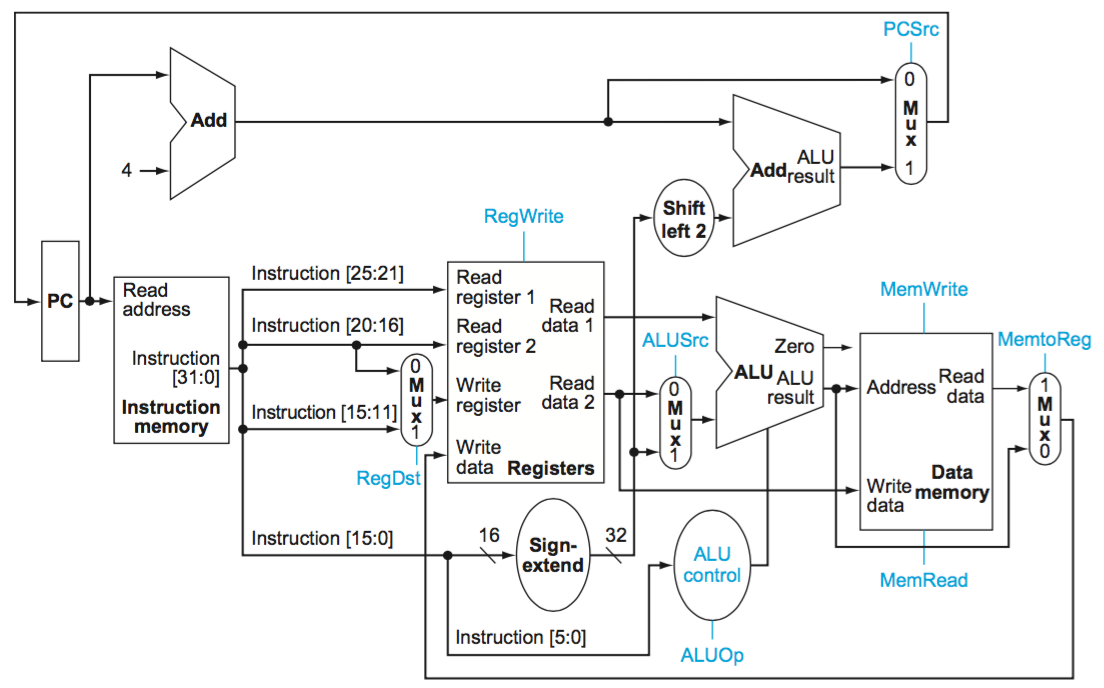
\includegraphics[angle=90, width=1.0\textwidth]{pictures/fullDataPath.png}
    \caption{Data-path with all necessary multiplexers and all control lines.}
    \label{fullDataPath}
  \end{figure}
  \newpage
  \section{A Simple Implementation Scheme}
  \subsection{The ALU Control}
  The MIPS ALU defined in ``Computer Organization and Design'' Appendix B defines the 6 following combinations of four control inputs:
  \begin{center}
  \begin{tabular} {c | c}
    ALU Control Lines & Function          \\ \hline
    0000              & AND               \\ \hline
    0001              & OR                \\ \hline
    0010              & add               \\ \hline
    0110              & subtract          \\ \hline
    0111              & set on less than  \\ \hline
    1100              & NOR               \\ \hline
  \end{tabular}
  \end{center}
  The ALU will need to perform one of the first five functions depending on the instruction class.
  NOR will be covered later. \\
  For load and store word instructions, ALU is used to compute the memory address by addition. \\
  For R-type instructions, ALU needs to perform AND, OR, subtract, add, or set on less than, depending on the value of the 6-bit function field in the low-order bits of the instruction. \\
  For branch equal, the ALU must perform a subtraction. \\

  In many instances, we do not care about the values of some of the \emph{inputs}, and because we wish to keep the tables compact, we also include \emph{don't-care terms}.
  A don't-care term in this truth table (represented by an X in an input column) indicates that the output does not depend on the value of the input corresponding to that column.

  \subsection{Designing the Main Control Unit}
  The three instruction classes (R-Type, load and store, and branch) use two different instruction formats; jump instructions use another format
  \begin{itemize}
    \item R-format instructions have an opcode of 0.
    They have three register operands: rs, rt, and rd.
    Fields rs and rt are sources, and rd is the destination.
    The ALU function is in the funct field and is decoded by the ALU control design.
    The shamt field is used only for shifts.
    \item Instruction format for load (opcode=35) and store (opcode=43) instructions.
    The register rs is the base register that is added to the 16-bit address field to form the memory address.
    For load, rt is the destination register for the loaded value.
    For stores, rt is the source register whose value should be stored in memory.
    \item Instruction format for branch equal (opcode=4).
    The registers rs and rt are the source registers that are compared for equality.
    The 16-bit address field is sign-extended, shifted, and added to the PC+4 to compute the branch target address
  \end{itemize}

  The general format of instructions are
  \begin{itemize}
    \item The op field, opcode, is always contained in bits 31:26.
    \item The two registers to be read are always specified by the rs and rt fields, at positions 25:21 and 20:16.
    This is true for the R-type instructions, branch equal, and store.
    \item The base register for load and store instruction is always in bit position 25:21 (rs).
    \item The 16-bit offset for branch equal, load, and store is always in positions 15:0.
    \item The destination register is in one of two places.
    For a load, it is in bit positions 20:16 (rt), while for an R-type instruction it is in bit positions 15:11 (rd).
    Thus, a multiplexer is added to select which field of the instruction is used to indicate the register number to be written.
  \end{itemize}

  The control unit can set all but one of the control signals based solely on the opcode field of the instruction.
  The PCSrc control line is the exception; that control line should be asserted if the instruction is branch on equal (a decision that the control unit can make) \emph{and} the Zero output of the ALU, which is used for equality comparison, is asserted. \\

  \textbf{Outputs for Control Unit} \\
  The output from the control unit are the control lines that:
  \begin{enumerate}
    \item Signal when memory should be write enabled (1-3)
    \item Signal when data lines a multiplexer show forward on (4-7)
    \item Signal which function the ALU should perform (8)
  \end{enumerate}
  \begin{tabular}{c || l | p{5cm} | l}
  & Signal/Outputs & If Signal == 1 & If Signal == 0 \\ \hline \hline
  1. & \emph{MemWrite} & Write to Data Memory & No effect \\ \hline
  2. & \emph{MemRead} & Memory read memory & No effect \\ \hline
  3. & \emph{RegWrite} & Write data to Register File & NO effect \\ \hline
  4. & \emph{MemtoReg} & Use data from Data Memory & Use ALUResult \\ \hline
  5. & \emph{Branch} & Use PCBranch result for PC & No branch; use PC + 4 \\ \hline
  6. & \emph{RegDst} & Use 15:11 field for write address (rd used) & Use 20:16 field (rt used) \\ \hline
  7. & \emph{ALUSrc} & Use immediate field from Instr & Use Register File \\ \hline
  8. & \emph{ALUControl\textsubscript{2:0}} &
  \multicolumn{2}{l}{Specify the ALU operation: add, sub, and, or}
  \end{tabular} \\

  The settings of the control lines is completely determined by the opcode fields of the instruction.
  \begin{multicols}{4}
  \begin{enumerate}
    \item R-Format
    \begin{enumerate}
      \item[RegDst] 1
      \item[ALUSrc] 0
      \item[MemtoReg] 0
      \item[RegWrite] 1
      \item[MemRead] 0
      \item[MemWrite] 0
      \item[Branch] 0
      \item[ALUOp1] 1
      \item[ALUOp0] 0
    \end{enumerate}
    \item lw
    \begin{enumerate}
      \item[RegDst] 0
      \item[ALUSrc] 1
      \item[MemtoReg] 1
      \item[RegWrite] 1
      \item[MemRead] 1
      \item[MemWrite] 0
      \item[Branch] 0
      \item[ALUOp1] 0
      \item[ALUOp0] 0
    \end{enumerate}
    \item sw
    \begin{enumerate}
      \item[RegDst] X
      \item[ALUSrc] 1
      \item[MemtoReg] X
      \item[RegWrite] 0
      \item[MemRead] 0
      \item[MemWrite] 1
      \item[Branch] 0
      \item[ALUOp1] 0
      \item[ALUOp0] 0
    \end{enumerate}
    \item beq
    \begin{enumerate}
      \item[RegDst] X
      \item[ALUSrc] 0
      \item[MemtoReg] X
      \item[RegWrite] 0
      \item[MemRead] 0
      \item[MemWrite] 0
      \item[Branch] 1
      \item[ALUOp1] 0
      \item[ALUOp0] 1
    \end{enumerate}
  \end{enumerate}
  \end{multicols}

  \textbf{ALU Decoder}
  How the main decoder signals the ALU decoder: \\
  \begin{tabular} {l | l}
  ALUOp\textsubscript{1:0} & Meaning \\ \hline \hline
  00 & Add \\ \hline
  01 & Subtract \\ \hline
  10 & Look at Funct \\ \hline
  11 & Not Used \\ \hline
  \end{tabular} \\

  The inputs (ALUOp\textsubscript{1:0} and Funct) and the output (ALUControl\textsubscript{2:0}): \\
  \begin{tabular}{l | l | l}
  ALUOp\textsubscript{1:0} & Funct Field & ALUControl\textsubscript{2:0} \\ \hline \hline
  00 & X & 010 (Add) \\ \hline
  X1 & X & 110 (Subtract) \\ \hline
  1X & 100000 (add) & 010 (Add) \\ \hline
  1X & 100010 (sub) & 110 (Subtract) \\ \hline
  1X & 100100 (and) & 000 (And) \\ \hline
  1X & 100101 (or) & 001 (Or)
  \end{tabular}

  \subsection{Procedure of Executing the Load Instruction}
  \begin{enumerate}
    \item[1] \emph{Fetch} the instruction, say \emph{lw \$2, 4(\$1)}
    \begin{enumerate}
      \item Start at the program counter (PC) to get the address of the next instruction
      \item Go the the \emph{Instruction Memory} to get next instruction
    \end{enumerate}
    \item[2a] Get the value stored in the \emph{Register File} at location \emph{\$1}
    \begin{enumerate}
      \item Specify the address (00001) at input A1 of the \emph{Register File}
      \item The data will appear at output RD1 of the \emph{Register File}
    \end{enumerate}
    \item[2b] \emph{Sign extend} the \emph{offset}
    \begin{enumerate}
      \item The offset, 4, is specified in the instruction
      \item Convert the offset from a 16-bit signed integer to a 32-bit signed integer by sign extending it
    \end{enumerate}
    \item[2c] Calculate the memory address of the data
    \begin{enumerate}
      \item Send the base address and the offset to inputs \emph{SrcA} and \emph{SrcB} of the \emph{Arithmetic Logic Unit} (ALU)
      \item Signal the \emph{ALU} to add the inputs with control signal \emph{ALUControl}
      \item The sum will appear at \emph{ALUResult}
    \end{enumerate}
    \item[2d] Read the data stored at this address
    \begin{enumerate}
      \item Send the memory address to the \emph{Data Memory}
      \item The data stored at that address will appear at output \emph{RD}
    \end{enumerate}
    \item[2e] Write the data into the \emph{Register File} at location \emph{\$2}
    \begin{enumerate}
      \item Send the \emph{ReadData} back to the \emph{Register File}
      \item Send the address (00010) to the \emph{Register File}
      \item Signal the \emph{Register File} to store the data (\emph{RegWrite}) at input \emph{WD3}
    \end{enumerate}
  \end{enumerate}

  \subsection{Why a Single-Cycle Implementation Is Not Used Today}
  It is inefficient because the clock cycle must have the same length for every instruction in single-cycle design. \\
  The longest possible path in the processor determines the clock cycle, which is the load instruction.
  It uses instruction memory, the register file, the ALU, the data memory, and the register file in series. \\

  There's significant drawback for using single-cycle design with a fixed clock cycle; but it may be considered acceptable for a small instruction set. \\
  It does not scale well when adding more complex instructions. \\
  It is not possible to improve the worst-case cycle time in a single-cycle design even if there are techniques to improve the common-case cycle time. \\

  Thus, we use pipelining to improve the efficiency and throughput.
  Pipelining improves efficiency by executing multiple instructions simultaneously.

  \section{An Overview of Pipelining}
  \emph{Pipelining} is an implementation technique in which multiple instructions are overlapped in execution. \\
  The idea to that all steps---called \emph{stages} in pipelining---are operating concurrently.
  As long as each stage has separate resources, the tasks can be pipelined. \\

  For pipelining MIPS instructions, each instruction classically takes five steps (stages):
  \begin{itemize}
    \item[1.] Fetch instruction from memory
    \item[2.] Read registers while decoding the instruction. The regular format of MIPS instructions allow reading and decoding to occur simultaneously.
    \item[3.] Execute the operation or calculate an address.
    \item[4.] Access an operand in data memory
    \item[5.] Write the result into a register
  \end{itemize}
  If the stages are perfectly balanced, then the time between instructions on the pipelined processor---assuming ideal condition---is equal to
  $$\text{Time between instructions}_\text{pipelined} = \frac{\text{Time between instruction}_\text{non-pipelined}}{\text{Number of pipe stages}}$$
  Under ideal condition and a large number of instruction, the performance is increased is approximately equal to the number of pipe stages. \\

  Pipelining improves performance \emph{increasing instruction throughput, as opposed to decreasing the execution time of an individual instruction}, but instruction throughput is the important metric because real programs execute billions of instruction.

  \subsection{Designing Instruction Sets for Pipelining}
  All MIPS instructions are the same length, which makes it easier to fetch instructions in the first pipeline stage and to decode them in the second stage. \\
  MIPS has only a few instruction formats, with the source register fields being located in the same place in each instruction. \\
  Thus, the second stage can begin reading the register file at the same time that the hardware is determining what type of instruction was fetched.
  If not for the symmetry in instruction formats, stage 2 would need to be split resulting in 6 pipeline stages (longer pipelines are not desired). \\
  In addition, memory operands only appear in loads or stores in MIPS.
  Which means we can use the execute stage to calculate the memory address and then access memory in the following stage.

  \subsection{Pipeline Hazards}
  Situations when the next instruction cannot execute in the following clock cycle are called \emph{hazards}.

  \subsubsection{Structural Hazard}
  A \emph{structural hazard} means the hardware cannot support the combination of instructions that we want to execute in the same clock cycle.

  \subsubsection{Data Hazard}
  A \emph{pipeline data hazard}, a form of \emph{data hazard}, occurs when the pipeline must be stalled because one step must wait for another to complete. \\
  In other words, a planned instruction cannot execute in the proper clock cycle because data that is needed to execute the instruction is not yet available. \\

  \emph{Forwarding}, also called \emph{bypassing}, is a method of solving a data hazard by retrieving the missing data element from internal buffers rather than waiting for it to arrive from programmer-visible register or memory. \\
  Forwarding paths are valid only if the destination stage is later in the time than the source stage. \\
  In other words, there cannot be a valid forwarding path from the output of the memory access stage in the first instruction to the input of the execution stage of the following, since that would mean going backward in time. \\

  A \emph{load-use data hazard} is a specific form of data hazard in which the data being loaded by a load instruction has not yet become available when it is needed by another instruction. \\
  A \emph{pipeline stall}, also called a \emph{bubble}, is a stall initiated in order to resolve a hazard.

  \subsubsection{Control Hazard}
  A \emph{control hazard}, also called \emph{branch hazard}, arises from the need to make a decision based on the results of one instruction while others are executing. \\
  This hazard comes from branch instructions as the pipeline cannot know the next possible instructions after fetching a branch instruction. \\
  Two ways to resolve control hazards:
  \begin{enumerate}
    \item \textbf{Stall} \\
      Stall immediately after a branch instruction is fetched, waiting until the pipeline determines the outcome of the branch and knows that instruction address to fetch from. \\
      If the branch cannot be resolved in the second stage, the cost of stalling is too high for most computes to use as it causes a even larger slowdown.
    \item \textbf{Predict} \\
      Computers use \emph{prediction} to handle branches.
      One approach is to predict always that branch will not be taken; when right,  the pipeline proceeds at full speed. \\
      If branch is taken, the pipeline stalls.
  \end{enumerate}

  A more sophisticated version of \emph{branch instruction} would have some branches predicted as taken and some as not taken. \\
  In programming, at the bottom of loops are branches that jump back to the top of the loop.
  Those branches are likely to be taken and they branch backwards, so it can be predicted as taken for branches that jump to an earlier address. \\
  \emph{Dynamic hardware predictors} make their guesses depending on the behavior of each branch and may change predictions for a branch over the life of a program.
  One approach is keeping a history for each branch as taken or not taken, and then using recent past history to predict the future. \\
  If prediction goes wrong, the pipeline control must ensure instructions following a wrongly guessed branch have no effect and must restart the pipeline from the proper branch address. \\

  A third approach to resolve control hazard is called \emph{delayed decision}, that's actually used in MIPS architecture.
  The delayed branch always execute the next sequential instruction, with the branch taking place after that one instruction delay.
  The assembler can automatically arrange the instructions to get the branch behavior desired by the programmer; it is hidden from the MIPS programmer.
  MIPS software places an instruction immediately after the delayed branch instruction that is not affected by the branch, and a taken branch changes the address of the instruction that follows this safe instruction. \\
  Delayed branches are useful when branches are short.
  Processors do not use a delayed branch of more than one cycle.
  For longer branch delays, hardware-based branch prediction is usually used.

  \subsection{Pipeline Overview Summary}
  Pipelining is a technique that exploits \emph{parallelism} among the instruction in a sequential instruction stream.
  Its substantial advantage is that it is fundamentally invisible to the programmer. \\
  Pipelining increases the number of simultaneously executing instructions and the rate at which instructions are started and completed.
  However, it does not reduce the time it takes to complete an individual instruction also called the \emph{latency}.
  \emph{Latency} in pipelining is the number of stages in a pipeline or the number of stages between two instruction during execution. \\
  Pipelining improves instruction \emph{throughput} rather than individual instruction \emph{execution time} or \emph{latency}.

  \section{Pipelined Datapath and Control}
  In a five-stage pipeline, up to five instructions will be in execution during any single clock cycle. \\
  The datapath can be separated into five pieces:
  \begin{enumerate}
    \item \textbf{IF}: Instruction fetch
    \item \textbf{ID}: Instruction decode and register file read
    \item \textbf{EX}: Execution or address calculation
    \item \textbf{MEM}: Data memory access
    \item \textbf{WB}: Write back
  \end{enumerate}
  For the register file and data memory units are split in two phases: write in the first half and read in the second half.

  \subsection{Pipelined Control}
  Only need to set the control values during each pipeline stage to specify control for the pipeline.
  Each control line is associated with a component active in only a single pipeline stage, thus the lines can be divided into five stages according to the pipeline stage.
  \begin{enumerate}
    \item \emph{Instruction fetch}:
    The control signals to read instruction memory and to write the PC are always asserted, so there is nothing special to control in this stage
    \item \emph{Instruction decode/register file read}:
    The same thing happens at every clock cycle, so there are not optional control lines to set.
    \item \emph{Execution/address calculation}:
    The signals to be set are \emph{RegDst}, \emph{ALUOp}, and \emph{ALUSrc}.
    The signals select the Result register, the ALU operation, and either Read data 2 or a sign-extended immediate for the ALU.
    \item \emph{Memory access}:
    The control lines set in this stage are \emph{Branch}, \emph{MemRead}, and \emph{MemWrite}.
    The branch equal, load, and store instructions set these signals respectively.
    Note that \emph{PCSrc} selects the next sequential address unless control asserts Branch and the ALU result was 0.
    \item \emph{Write back}:
    The two control lines are \emph{MemtoReg}, which decides between sending the ALU result or the memory value to the register file, and \emph{RegWrite}, which writes the chosen value.
  \end{enumerate}
  Implementing control means setting the nine control lines to these values in each stage for each instruction.
  The simple approach is to extend the pipeline registers to include control information. \\
  The control lines start with the \emph{EX} stage, so the control information can be created during instruction decode.

  \section{Data Hazards: Forwarding versus Stalling}
  The write is in the first half of the clock and the read is in the second half when a register is read and written in the same clock cycle.
  Thus, the read delivers what is written; this is a common implementation for register files. \\

  If the data is needed at the beginning of the EX stage, the data can be \emph{forwarded} as soon as it is available to any units that need it before the data is available in register file. \\
  For now, the only challenge of forwarding is to make the data available in an operation in the EX stage, which may either be an ALU operation or an effective address calculation.
  The two pairs of hazard conditions are:
  \begin{enumerate}
    \item[1a] EX/MEM.RegisterRd = ID/EX.RegisterRs
    \item[1b] EX/MEM.RegisterRd = ID/EX.RegisterRt
    \item[2a] MEM/WB.RegisterRd = ID/EX.RegisterRs
    \item[2b] MEM/WB.RegisterRd = ID/EX.RegisterRs
  \end{enumerate}

  \begin{ex}
    Suppose we have the following instructions sequence
    \begin{verbatim}
      sub $2,  $1, $3
      and $12, $2, $5
      or  $13, $6, $2
    \end{verbatim}
    Then sub-and is a type 1a hazard (EX/MEM.RegisterRd = ID/EX.RegisterRs)
    Whereas sub-or is a type 2b hazard (MEM/WB.RegisterRd = ID/EX.RegisterRs)
  \end{ex}
  This forwarding may not always work because some instructions do not write registers;
  sometimes it would forward when it shouldn't. \\
  A simple solution is to check if \emph{RegWrite} signal will be active: examining the WB control field of the pipelining register during the EX and MEM stages determines whether \emph{RegWrite} is asserted. \\
  Note that MIPS require every use of \$0 as an operand must yield an operand value of 0.
  Thus, need to avoid forwarding a possible non-zero value of \$0 in the event that \$0 is used as the destination.
  Thus, the conditions above work if EX/MEM.RegisterRd $\not =$ 0 and MEM/WB.RegisterRd $\not =$ 0.

  A new hardware, called \emph{Forwarding Unit} is added in the EX stage to expand the multiplexers into the ALU unit such that it can take in the forwarded data.
  \begin{center}
  \begin{tabular}{l | l | p{9cm}}
    Mux Control & Source & Explanation \\ \hline \hline
    ForwardA = 00 & ID/EX   & The first ALU operand comes from the register file \\ \hline
    ForwardA = 10 & EX/MEM  & The first ALU operand is forwarded from the prior ALU result. \\ \hline
    ForwardA = 01 & MEM/WB  & The first ALU is forwarded from data memory or an earlier ALU result \\ \hline
    ForwardB = 00 & ID/EX   & The second ALU operand comes from the register file \\ \hline
    ForwardB = 10 & EX/MEM  & The second ALU operand is forwarded from the prior ALU result. \\ \hline
    ForwardB = 01 & MEM/WB  & The second ALU is forwarded from data memory or an earlier ALU result \\ \hline
  \end{tabular}
  \end{center}
  Note that the EX/MEM.RegisterRd field is the register destination for either an ALU instruction (which comes from the Rd field of the instruction) or a load (which comes from the Rt field).
  \begin{enumerate}
    \item \emph{EX Hazard}
\begin{verbatim}
if (EX/MEM.RegWrite
and (EX/MEM.RegisterRd != 0)
and (EX/MEM.RegisterRd = ID/EX.RegisterRs))   ForwardA = 10

if (EX/MEM.RegWrite
and (EX/MEM.RegisterRd != 0)
and (EX/MEM.RegisterRd = ID/EX.RegisterRt))   ForwardB = 10
\end{verbatim}
    \item \emph{MEM Hazard}
\begin{verbatim}
if (MEM/WB.RegWrite
and (MEM/WB.RegisterRd != 0)
and not(EX/MEM.RegWrite and (EX/MEM.RegisterRd != 0)
      and (EX/MEM.RegisterRd != ID/EX.RegisterRs))
and (MEM/WB.RegisterRd = ID/EX.RegisterRs))   ForwardA = 01

if (MEM/WB.RegWrite
and (MEM/WB.RegisterRd != 0)
and not(EX/MEM.RegWrite and (EX/MEM.RegisterRd != 0)
      and (EX/MEM.RegisterRd != ID/EX.RegisterRt))
and (MEM/WB.RegisterRd = ID/EX.RegisterRt))   ForwardB = 01
\end{verbatim}
  \end{enumerate}

  \subsection{Data Hazards and Stalls}
  A particular case when forwarding does not work is when an instruction tries to read a register following a load instruction that writes the same register. \\
  In addition to a forwarding unit, we need a \emph{hazard detection unit} such that it can stall the pipeline.
  It is to operate during the ID stage so that it can insert the stall between the load and its use.
  \begin{verbatim}
  if (ID/EX.MemRead and
      ((ID/EX.RegisterRt = IF/ID.RegisterRs) or
        (ID/EX.RegisterRt = IF/ID.RegisterRt)))
        stall the pipeline
  \end{verbatim}
  The first line tests to see if the instruction is a load: the only instruction that reads data memory is a load.
  The next two lines check to see if the destination register field of the load in the EX stage matches either source register of the instruction in the ID stage. \\

  If the instruction in the ID stage is stalled, then the instruction in the IF stage must also be stalled;
  otherwise, we would lose the fetch instruction.
  So we execute instructions that have no effects: \emph{nops}.
  ``nop'' is an instruction that does no operation to change state.
  This way, the appropriate instructions can be stalled while depended instructions execute. \\

  By setting all nine control signals to 0 in the EX, MEM, and WB stages will create a ``do nothing'' or nop instruction. \\
  When the hazard is identified in the ID stage, a bubble can be inserted into the pipeline by changing the EX, MEM, and WB control fields of the ID/EX pipeline register to 0.
  No registers or memories are written if the control values are all 0. \\

  \begin{figure}[!ht]
  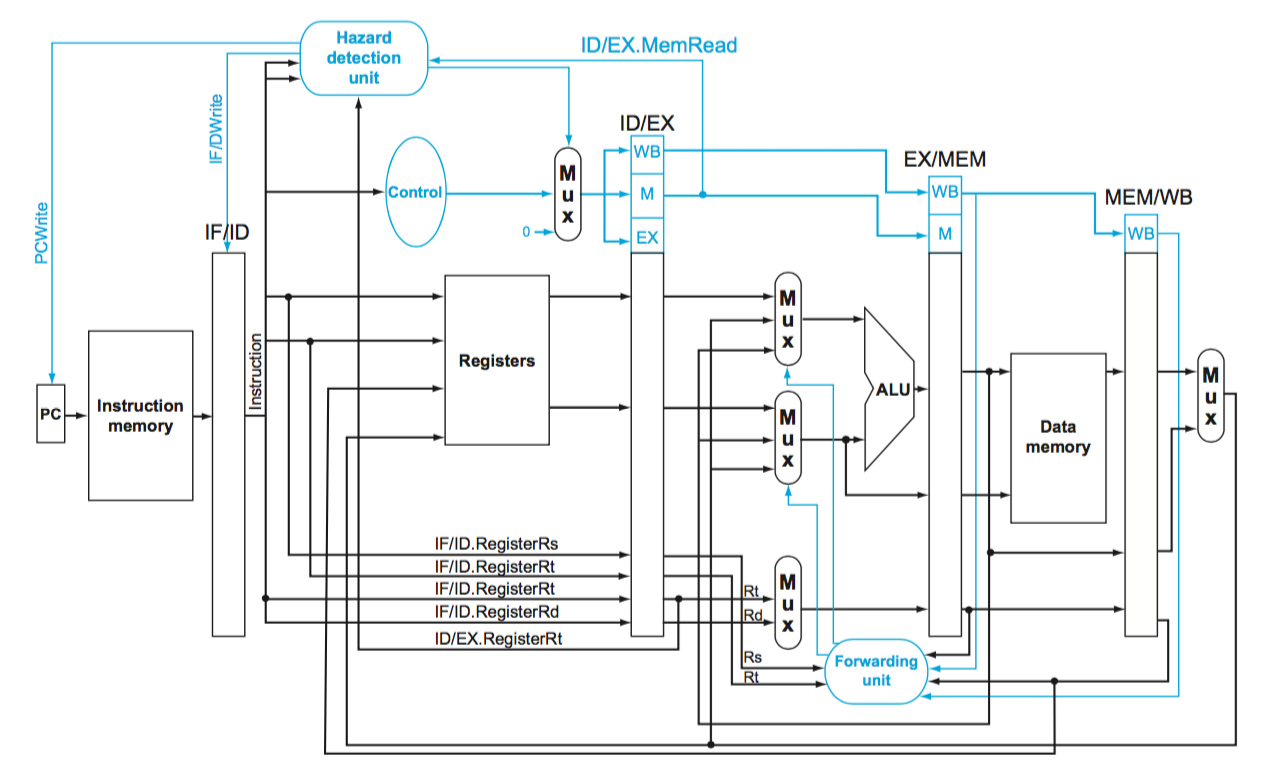
\includegraphics[width=1.0\textwidth]{pictures/hazardAndForwardingUnits.png}
  \caption{Implementation of Stalling and Forwarding}
  \end{figure}

  The \emph{hazard detection unit} controls the the writing of the PC and IF/ID registers plus the multiplexer that chooses between the real control values and all 0s. \\
  The unit stalls and deasserts the control fields if the load-use hazard test is true.

  \section{Control Hazards} % 4.8 in P+H
  An instruction must be fetched at every clock cycle to sustain the pipeline, the decision to branch does not occur until the MEM pipeline stage.
  This delay in determining the proper instruction to fetch is a \emph{control hazard} or \emph{branch hazard}. \\
  There are two schemes for resolving control hazards and one optimization to improve these schemes.
  \subsection{Assume Branch Not Taken}
  Stalling until the branch is complete is slow.
  An improvement is to \textbf{predict} that the branch will not be taken and thus continue execution down the sequential instruction stream. \\
  If branch is taken, the instructions that are being fetched and decoded must be discarded;
  execution continues at the branch target. \\
  If branches are not taken half the time, and if it costs little to discard the instructions, this method of optimization halves the cost of control hazards. \\

  To discard instructions, the original control values are changed to 0s, akin to stall a load-use data hazard. \\
  Note that all three instructions in the IF, ID, and EX stages need to be changed when the branch reaches the MEM stage;
  whereas only the controls in TD stage are changed to 0 and let them percolate through the pipeline. \\
  To discard instructions, the instructions in the IF, ID, and EX stages must be \textbf{flushed}.

  \subsection{Reducing the Delay of Branches}
  Another improvement is to reduce the cost of the taken branch.
  If branch execution is moved to an earlier stage in the pipeline, instead of MEM stage, then fewer instructions need to be flushed. \\
  Many branches rely only on simple tests that do not require a full ALU operation, it can be done with at most a few gates.
  If a more complex branch decision is needed, a separate instruction that uses an ALU is required. \\

  Moving the branch decision up requires two actions to occur earlier, and their respective complications:
  \begin{enumerate}
    \item Computing the branch target address
    \begin{itemize}
      \item The PC value and the immediate field are available in the IF/ID register.
      \item The branch adder can be moved from the EX stage to the ID stage.
      \item Note that the branch target address calculation will be performed for all instructions, but it will only be used when needed.
    \end{itemize}
    \item Evaluating the branch decision
    \begin{itemize}
      \item Moving the branch test to the ID stage implies additional forwarding and hazard detection hardware, since a branch dependent on a result still in the pipeline must work properly with this optimization.
      \item During ID: must decode the instruction, decide whether a bypass to the equality unit is required, and complete the comparison to set the PC if it is a branch instruction.
      \item A new forwarding logic is required for the equality test unit in ID. \\
      Bypassed source operands of a branch can come from either the ALU/MEM or MEM/WB pipeline latches.
      \item A data hazard can occur and a stall is needed if the values in a branch comparison are produced later in time.
    \end{itemize}
  \end{enumerate}
  The improvement of moving the branch execution to the ID stage is that the penalty of a branch is reduced to only one instruction if the branch is taken (the one being fetched in IF stage). \\
  To flush instructions in the IF stage, a control line named \emph{IF.Flush} zeros the instruction field of the IF/ID pipeline register. \\
  Clearing the register transforms the fetched instruction into a \textbf{nop}, an instruction that has no action and changes no state.

  \subsection{Dynamic Branch Prediction}
  Assuming a branch is not taken is a form of \emph{branch prediction}.
  It is probably adequate for a simple five-stage pipeline, and possibly coupled with compiler-based prediction.
  With more complex pipelines, the branch penalty increases when measured in clock cycles and it increases in terms of instructions lost.
  A simple static prediction scheme will waste too much performance in complex pipelines. \\

  \emph{Dynamic branch prediction} is to look up the address of the instruction to see if a branch was taken the last time this instruction was executed, and if so, to begin fetching new instructions from the same place as the last time. \\
  One implementation is a \emph{branch prediction buffer} and \emph{branch history table}.
  The buffer is a small memory indexed by the lower portion of the address of the branch instruction.
  This memory contains a bit that says whether the branch was recently taken or not. \\

  It is possible that the prediction is correct; another branch instruction could have used the same lower-order address bits. \\
  However, predicting is a hint that we hope is correct, so fetching begins in the predicted direction.
  Thus, it does not affect the correctness of the predictions. \\
  In the event that the hint is wrong, the incorrectly predicted instructions are deleted, the prediction bit is inverted and stored back. and the proper sequence is fetched and executed. \\

  A shortcoming of a 1-bit prediction scheme is that: even if a branch is almost always taken (ex. loop), the prediction can wrong twice, rather than once, when it's not taken. \\

  To remedy the weakness of poor accuracy of 1-bit prediction schemes, 2-bit prediction schemes are often used.
  A prediction must be wrong twice before it is changed in a 2-bit scheme. \\

  A branch prediction buffer can be implemented as a small special buffer accessed with the instruction address during the IF pipe stage. \\
  If the instruction is predicted as taken, fetching begins from the target as soon as the PC is known. \\
  Otherwise, sequential fetching and executing continue. \\
  If the prediction is wrong, the prediction bits are changed. \\

  \textbf{Elaboration}: \\
  A delayed branch always executes the following instruction, but the second instruction following the branch will be affected by the branch.
  Compilers and assemblers try to place an instruction that always executes after the branch in the \emph{branch delay slot}. \\

  \textbf{Elaboration}: \\
  A branch predictor tells whether or not a branch is taken, but still requires the calculation of the branch target.
  The calculation takes one cycle, which means that taken branches have a 1-cycle penalty. \\
  The penalty can be resolved by delayed branches or through a \emph{branch target buffer}.
  A branch target buffer is a structure that caches the destination PC or destination instruction for a branch.
  It is usually organized as a cache with tags, thus more costly than a simple prediction buffer.\\

  The 2-bit dynamic prediction scheme uses only information about a particular branch.
  However, using information about both a local branch, and the global behavior of recently executed branches together yields greater prediction accuracy for the same number of prediction bits.
  This is a \emph{correlating predictor}. \\
  A typical correlating predictor have two 2-bit predictors for each branch, with the choice between predictors made based on whether the last executed branch was taken or not.
  Thus, the global branch behavior can be thought as an adding additional index bits for the prediction lookup. \\

  A recent innovation in branch predicting is the use of tournament predictors. \\
  A \emph{tournament predictor} uses multiple predictors, tracking, for each branch, which predictor yields the best results.
  A typical one might contain two predictions for each branch index: one based on local information and the other based on global branch behavior. \\
  A selector would choose which predictor to use for any given prediction.
  The selector can operate similarly to a 1- or 2-bit predictor, favoring whichever of the two has been more accurate.

  \begin{figure}
  \centering
  \caption{The final datapath and control}
  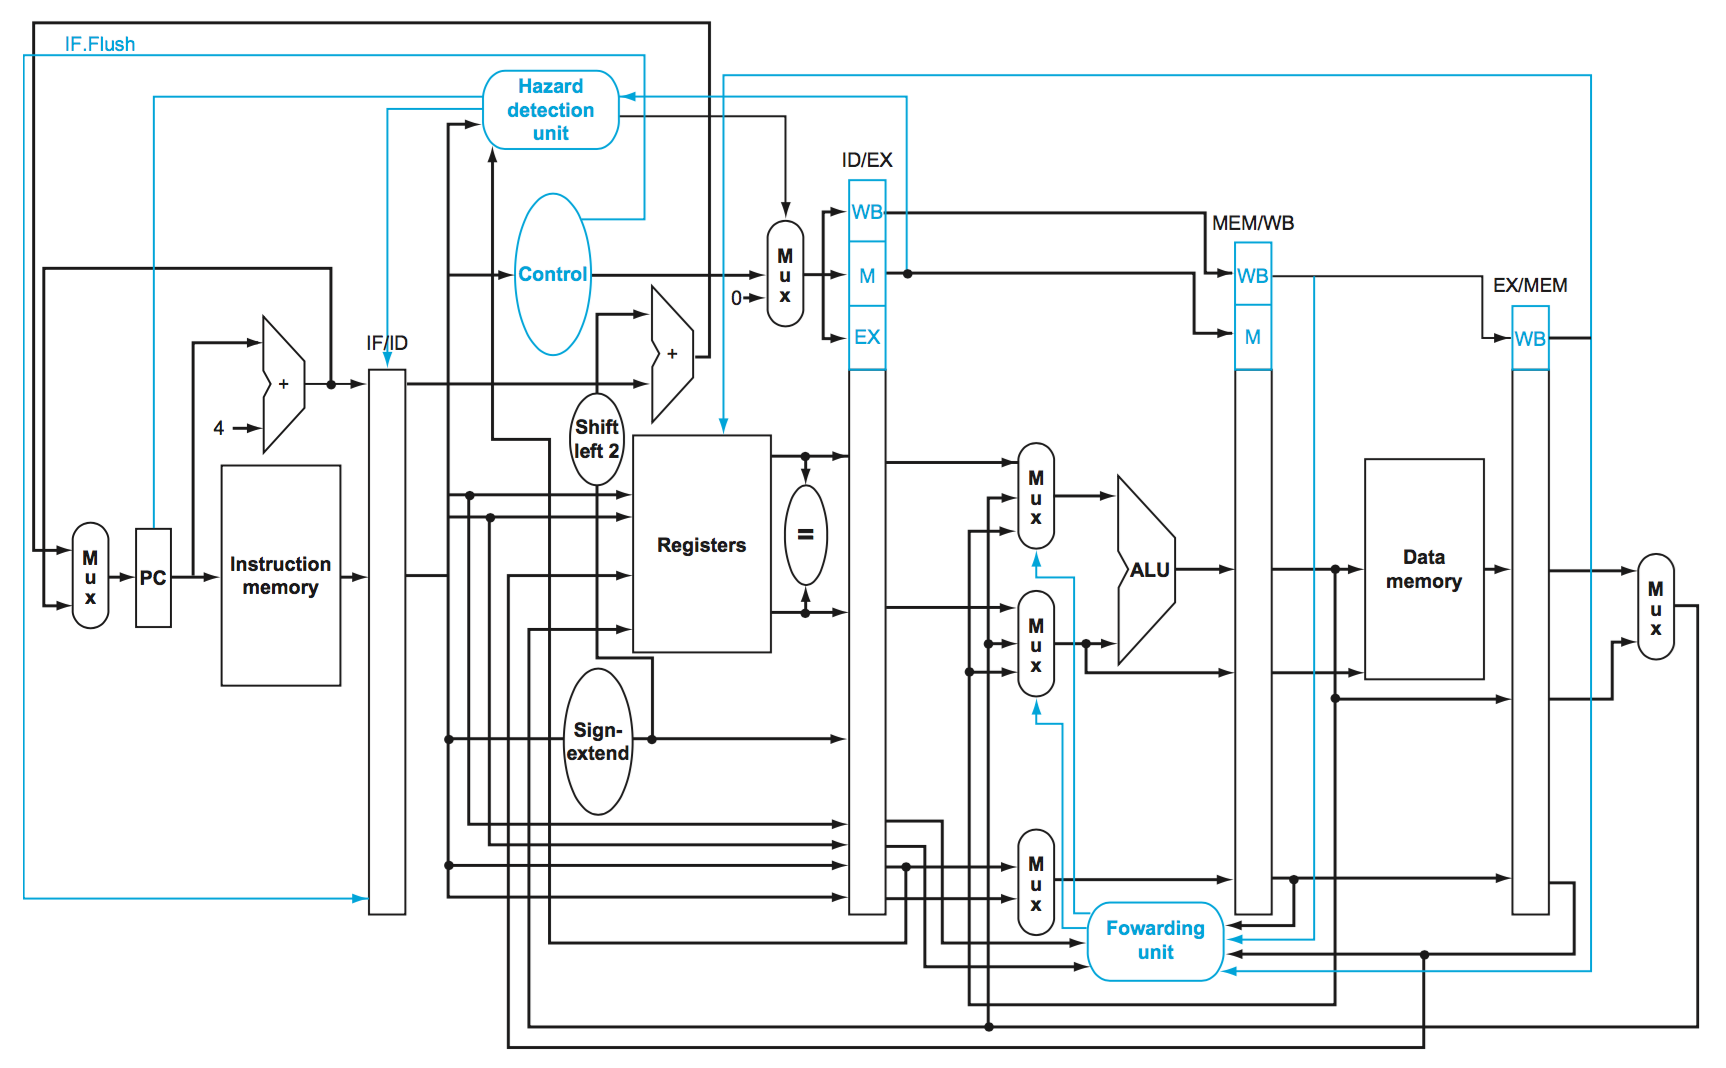
\includegraphics[width=1.0\textwidth]{pictures/finalPipelineDataPath.png}
  \end{figure}

  \section{Exceptions}
  Control is the most challenging aspect of processor design: it is both the hardest part to get right and the hardest part to make fast.
  One of the hardest parts of control is implementing \emph{exceptions} and \emph{interrupts}. \\
  An \emph{exception}, also called \emph{interrupt}, is an unscheduled event that disrupts program execution; used to detect overflows.
  An \emph{interrupt} is an exception that comes from outside of the processor.
  Initially created to handle unexpected events from within the processor, like arithmetic overflow. \\

  Detecting exceptional conditions and taking the appropriate action is often on the critical timing path of a processor, which determines the clock cycle time and thus performance. \\
  Without proper attention to exceptions during design of the control unit, attempts to add exceptions to a complicated implementation can significantly reduce performance, as well as complicate the task of getting the correct design.

  \subsection{How Exceptions Are Handled in the MIPS Architecture}
  The basic action that the processor must perform when an exception occurs is to save the address of the offending instruction in the \emph{exception program counter} (EPC) and then transfer control to the operating system at some specified address. \\

  The operating system (OS) can then take the appropriate action, which may involve providing some service to the user program, taking some predefined action in response to an overflow, or stopping the execution of the program and reporting an error. \\
  After performing the correct action is required due to the exception, the OS can terminate the program or may continue its execution, using the EPC to determine where to restart the execution of the program. \\

  For the OS to handle an exception, it must know the reason and the instruction that cause it. \\
  Two main methods to communicate the reason for an exception:
  \begin{enumerate}
    \item Include a status register (called the \emph{Cause Register}), which holds a field that indicates the reason for the exception.
    \item Use \emph{vectored interrupts}. In a vectored interrupt, the address to which control is transferred is determined by the cause of the exception. \\
    Ex. Type: undefined instruction; Vector address: 8000 0000\textsubscript{hex}
  \end{enumerate}

  The OS knows the reason for the exception by the address at which it is initiated.
  The addresses are separated by 32 bytes or eight instructions, and the OS must record the reason for the exception and may perform some limited processing in this sequence. \\
  When the exception is not vectored, a single entry point for all exceptions can be used, and the OS decodes the status register to find the cause. \\

  Two additional registers must be added to the MIPS implementation we have so far:
  \begin{itemize}
    \item[\emph{EPC}] A 32-bit register used to hold the address of the affected instruction. \\
    Such a register is needed even when exceptions are vectored.
    \item[\emph{Cause}] A register used to record the cause of the exception.
    In the MIPS architecture, this register is 32 bits, although some bits are unused.
  \end{itemize}

  \subsection{Exceptions in a Pipelined Implementation}
  A pipelined implementation treats exceptions as another form of control hazard.
  We will use the same mechanism used for taken branches, but this time the exception causes the deasserting of control lines. \\

  When dealing with branch mis-predict, the instruction in the IF stage is flushed by turning it into a \emph{nop}. \\
  To flush instructions in the ID stage, we use the multiplexer already in the ID stage that zeros control signals for stalls.
  A new control signal, called \emph{ID.Flush}, is ORed with the stall signal from the hazard detection unit to flush during ID. \\
  To flush instruction in the EX stage, a new signal called \emph{EX.Flush} is used to cause new multiplexers zero the control lines. \\
  Then we start fetching instructions from location 8000 0180\textsubscript{hex}, which is the MIPS exception address, we simply add an additional input to the PC multiplexer to send the address to the PC.

  \begin{figure}[!ht]
    \center{
      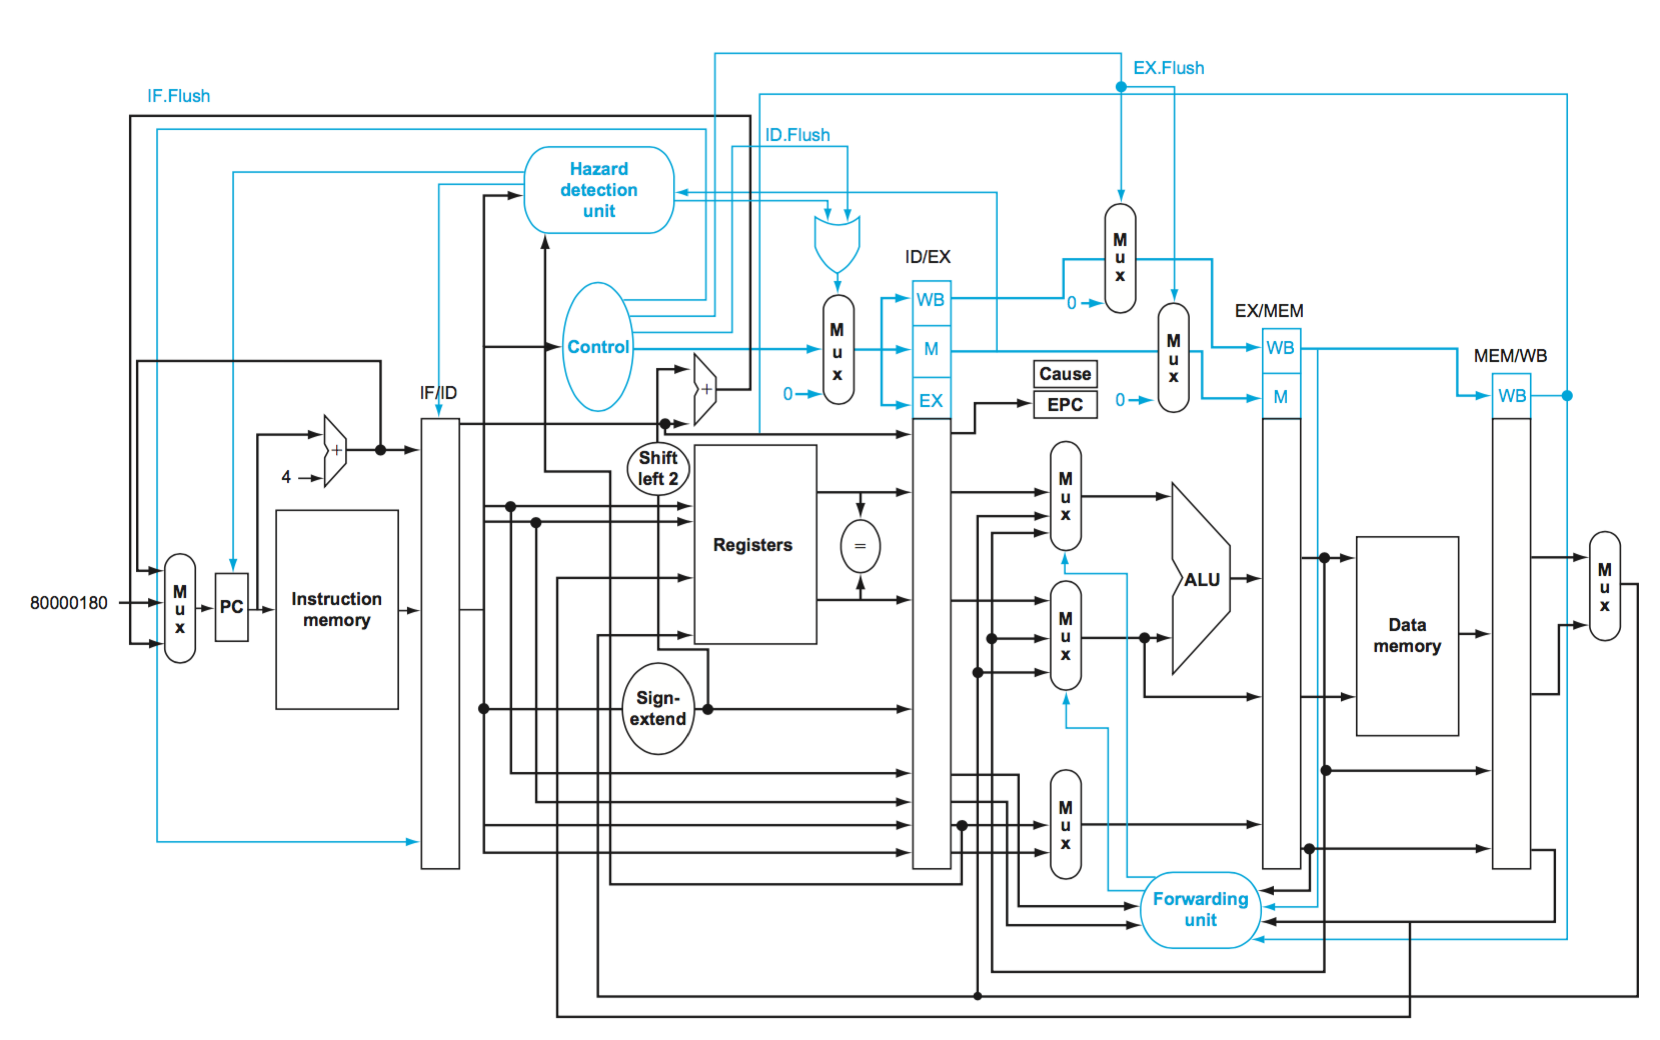
\includegraphics[width=1.0\textwidth]{pictures/datapathWithExceptions.png}
      \caption{The datapath with controls to handle exceptions}
    }
  \end{figure}

  Many exceptions require that we eventually complete the instruction that caused the exception as if it executed normally.
  The easiest way to do this is to flush the instruction and restart it from the beginning after the exception is handled. \\

  The final step is to save the address of the offending instruction in the \emph{exception program counter} (EPC).
  In reality, we save the address + 4, so the exception handling the software routine must subtract 4 from the saved value. \\

  Multiple exceptions can occur simultaneously in a single clock cycle.
  The solution is to prioritize the exceptions so that it is easy to determine which is serviced first.
  In most MIPS implementations, the hardware sorts exception so that the earliest instruction is interrupted. \\
  I/O device requests and hardware malfunctions are not associated with a specific instruction, so that implementation has some flexibility as to when to interrupt the pipeline. \\

  The EPC (exception program counter) captures the address of the interrupted instructions, and the MIPS Cause Register records all possible exceptions in a clock cycle, so the exception software must match the exception to the instruction.
  An important clue is knowing in which pipeline stage a type of exception can occur. \\
  Exceptions are collected in the Cause Register in a pending exception field so that the hardware can interrupt based on later exceptions, once the earliest one has been serviced.

  \subsection{Hardware/Software Interface}
  The hardware and the OS must work together so that exceptions behave as expected. \\

  The hardware contract is normally to stop the offending instruction in midstream, let all prior instructions complete, flush all following instructions, set a register to show the cause of the exception, save the address of the offending instruction, and then jump to a prearranged address. \\

  The OS contract is to look at the cause of the exception and act appropriately. \\
  For an undefined instruction, hardware failure, or arithmetic overflow exception, the operating system typically terminates the program and returns an indicator of the reason. \\
  For an I/O device request or an OS service call, the system saves the state of the program, performs the desired task, and, at some point in the future, restores the program to continue execution.
  We often choose to run another task before resuming the task that requested the I/O, since that task may often not be able to proceed until the I/O is complete. \\

  Exceptions are why the ability to save and restore the state of any task is critical. \\

  The difficulty of always associating the correct exception with the correct instruction in pipelined computers has led some computer designers to relax this requirement in noncritical cases.
  Such processors are said to have \emph{imprecise interrupts} or \emph{imprecise exceptions},
  which are interrupts/exceptions that are not associated with the exact instruction that was the cause. \\
  MIPS and the vast majority of computers today support \emph{precise interrupts} or \emph{precise exceptions}, which are interrupts/exceptions that are associated with the correct instruction.

  \section{Introduction to Large and Fast: Exploiting Memory Hierarchy}
  The \emph{principle of locality} states that programs access a relatively small portion of their address space at any instant of time. \\
  There are two different types of locality:
  \begin{enumerate}
    \item \textbf{Temporal Locality} (locality in time): if an item is referenced, it will tend to be referenced again soon.
    \item \textbf{Spatial Locality} (locality in space): if an item is referenced, items whose addresses are close by will tend to be referenced soon.
  \end{enumerate}
  Locality in programs arises from simple and natural program structures.
  For example, most programs contain loops, so instructions and data are likely to be accessed repeatedly, showing high amounts of temporal locality.
  In addition, those instructions are normally accessed sequentially, programs also show high spatial locality. \\

  We can take advantage of the principle of locality by implementing the memory of computer as a \emph{memory hierarchy}.
  A memory hierarchy consists of multiple levels of memory with different speeds and sizes.
  The faster memories are more expensive per bit than the slower memories and thus are smaller.
  As distance from the processor increases, the size of the memories and the access time both increases. \\

  The data is similarly hierarchical: a level closer to the processor is generally a subset of any level further away, and all the data is stored at the lowest level (hard disk).
  A memory hierarchy can consist of multiple levels, but data is copied between only two adjacent levels at a time, so we ca n focus out attention on just two levels.
  The upper level---the closer to the processor---is smaller and faster than the lower level, since the upper level uses technology that is more expensive.
  The minimum unit of information that can be either present or not present in the two-level hierarchy is called a \emph{block} or a \emph{line}. \\

  If the data requested by the processor appears in some block in the upper level, this is a \emph{hit}. \\
  If the data is not found in the upper level, the request is called a \emph{miss}.
  Th lower level in the hierarchy is then accessed to retrieve the block containing the requested data. \\
  The \emph{hit rate}, or \emph{hit ratio}, is the fraction of memory accesses found in the upper level; it is often used as a measure of the performance of the memory hierarchy. \\
  The \emph{miss rate} (1-hit rate) is the fraction of memory access not found in the upper level. \\

  Performance is the major reason for having a memory hierarchy, the time to service hits and misses is important. \\
  \emph{Hit time} is the time to access the upper level of the memory hierarchy, which includes the time needed to determine whether the access is a hit or a miss. \\
  The \emph{miss penalty} is the time to replace a block in the upper level with the corresponding block from the lower level, plus the time to deliver this block to the processor. \\
  Since the upper level is smaller and built using faster memory parts, the hit time will be much smaller than the time to access the next level in the hierarchy, which is the major component of the miss penalty.

  \section{Memory Technologies}
  There are four primary technologies used in memory hierarchies. \\
  Main memory is implemented from DRAM (dynamic random access memory), while levels closer the processor (caches) uses SRAM (static random access memory). \\
  DRAM is less costly per bit than SRAM, although it is substantially slower.
  The price difference arises because DRAM uses significantly less area per bit of memory, and DRAMs thus have larger capacity for the same amount of silicon. \\

  \subsection{SRAM Technology}
  SRAMs are simply integrated circuits that are memory arrays with (usually) a single access port that can provide either a read or a write. \\
  SRAMs have a fixed access time to any datum, though read and write access times may differ. \\
  SRAMs don't need to refresh and so the access time is very close to the cycle time. \\
  SRAMs typically use six to eight transistors per bit to prevent the information from being disturbed when read. \\
  SRAM needs only minimal power to retain the charge in standby mode.

  \subsection{DRAM Technology}
  In a SRAM, as long as power is applied, the value can be kept indefinitely. \\
  In a dynamic RAM, the value kept in a cell is stored as a charge in a capacitor.
  A single transistor is then used to access this stored charge, either to read the value or to overwrite the charge stored there. \\
  Because DRAMs use only a single transistors per bit of storage, they are much denser and cheaper per bit than SRAM. \\
  As DRAMs store the charge on a capacitor, it cannot be kept indefinitely and must periodically be refreshed.
  Hence this memory structure is dynamic, as opposed to the static storage in an SRAM cell. \\

  To refresh the cell, we merely read its contents and write it back.
  The charge can be kept for several ms.
  If every bit had to be read out of the DRAM and then written back individually, the DRAM would be constantly refreshed, leaving no time to access it. \\
  DRAMs use a two-level decoding structure, which allows the ability to refresh an entire \emph{row} (which shares a word line) with a read cycle followed immediately by a write cycle. \\

  The row organization that helps with refresh also helps with performance.
  To improve performance, DRAMs buffer rows for repeated access.
  The buffer acts like a SRAM; by changing the address, random bits can be accessed in the buffer until the next row access.
  This capability improves the access time significantly, since the access time to bits in the row is much lower.
  When the row is in the buffer, it can be transferred by successive addresses at whatever the width of the DRAM is, or by specifying a block transfer and the starting address within the buffer. \\

  To further improve the interface to processors, DRAMs added clocks which is called Synchronous DRAMs or SDRAMs.
  The advantage is that the use of a clock eliminates the time for the memory and processor to synchronize.
  The speed advantage of synchronous DRAMs come from the ability to transfer the bits in the burst without having to specify additional address bits.
  Instead, the clock transfer the successive bits in a burst. \\
  \emph{Double Data Rate} (DDR) SDRAM is the fastest currently available.
  Data transfer on both the rising and falling edge of the clock, thereby getting twice as much bandwidth based on the clock rate and the data width. \\

  Sustaining the bandwidth requires clever organization \emph{inside} the DRAM.
  The DRAM can be internally organized, instead of just a faster row buffer, to read or write from multiple \emph{banks}, which each having its own row buffer.
  Sending an address to several banks permits them all to read or write simultaneously.
  The rotating access scheme is called \emph{address interleaving}. \\

  Memory for servers are commonly sold on small boards called \emph{dual inline memory modules} (DIMMs).
  SIMMs typically contain 4 to 16 DRAMs, and they are normally organized to be 8 bytes wide for server systems.

  \subsection{Flash Memory}
  Flash memory is a type of \emph{electrically erasable programmable read-only memory} (EEPROM). \\
  Unlike disks and DRAM, writes can wear out flash memory bits.
  To cope with such limits, most flash products include a controller to spread the writes by remapping blocks that have been written many times to less trodden blocks;
  this is called \emph{wear leveling}.
  Wear leveling lowers the potential performance of flash, but is is needed unless higher-level software monitors block wear.
  Flash controllers that perform wear leveling can also improve yield by mapping out memory cells that were manufactured incorrectly.

  \subsection{Disk Memory}
  A magnetic hard disk consists of a collection of platters, which rotate on a spindle at 5,400 to 15,000 revolutions per minute. \\
  To read and write information on a hard disk, a movable arm containing a small electromagnetic coil called a \emph{read-write head} is located just above each surface.
  The entire drive is permanently sealed to control the environment inside the drive, which, in turn, allows the disk heads to be much closer to the drive surface. \\

  Each disk surface is divided into concentric circles, called \emph{tracks}.
  These are typically tens of thousands of tracks per surface.
  Each track is in turn divided into \emph{sectors} that contain the information; each track may have thousands of sectors. \\
  Sectors are usually 512 to 4096 bytes in size.
  The sequence recorded on the magnetic media is a sector number, a gap, the information for that sector including error correction code, a gap, the sector number of the next sector, and so on. \\

  \subsubection{Accessing Data in a Hard Disk}
  To access data, the OS must direct the disk through a three-stage process. \\

  The first step is to position the head over the proper track.
  This operation is called a \emph{seek}, and the time to move the head to the desired track is called the \emph{seek time}. \\

  Once the head has reached the correct rack, we must wait for the desired sector to rotate under the read/write head. This time is called the \emph{rotational latency} or \emph{rotational delay}.
  The average latency to the desired information is halfway around the disk. \\

  The last component of a disk access, \emph{transfer time}, is the time to transfer a block of bits.
  The transfer time is a function of the sector size, the rotation speed, and the recording density of a track.

  \section{The Basics of Caches}
  \emph{Cache} represents the level of memory hierarchy between the processor and main memory.
  Cache is also used to refer to any storage managed to take advantage of locality of access. \\

  The simplest way to assign a location in the cache for each word in memory is to assign the cache location based on the \emph{address} of the word in memory.
  This cache structure is called \emph{direct-mapped}, since each memory location is mapped directly to exactly one location in the cache. \\
  The typical mapping between addresses and cache locations for a direct-mapped cache is usually simple.
  Almost all direct-cache mapped caches uses the following mapping to find a block:
  $$\text{(Block address) modulo (Number of blocks in the cache)}$$

  Each cache location can contain the contents of a number of different locations, but how do we know whether a requested word is in the cache or not?
  Thus, a set of \emph{tags} is added to the cache.
  The tags contain the address information required to identity whether a word in the cache corresponds to the requested word.
  The tag needs only to contain the upper portion of the address, corresponding to the bits that are not sued as an index into the cache. \\
  Architects omit the index bits due to redundancy, since by definition the index field of any address of a cache block must be that block number. \\

  We also need a way to recognize that a cache block does not have valid information.
  The most common method is to add a \emph{valid bit} to indicate whether an entry contains a valid address.
  If the bit is not set, there cannot be a match for this block. \\

  Caching is possibly the most important example of the big idea of \emph{prediction}.
  It relies on the principle of locality to try to find the desired data in the higher levels of the memory hierarchy, and provides mechanisms to ensure that when the prediction is wrong it finds and uses the proper data from the lower levels of memory hierarchy.
  The hit rates of the cache prediction on modern computers are often higher than 95\%.

  \subsection{Accessing a Cache}
  Suppose we have the following example of nine memory references to an empty eight-block cache.
  Since there are eight blocks in the cache, the lower-order three bits of an address give the block number:
  \begin{center}
  \begin{tabular}{| c | c | c | c |}
  \hline
  Decimal Address & Binary Address & Hit or Miss & Assigned Cache \\ \hline
  22 & 10110\textsubscript{two} & miss & (10\textcolor{blue}{110}\textsubscript{two} mod 8) = \textcolor{blue}{110}\textsubscript{two} \\ \hline
  26 & 11010\textsubscript{two} & miss & (11\textcolor{blue}{010}\textsubscript{two} mod 8) = \textcolor{blue}{010}\textsubscript{two} \\ \hline
  22 & 10110\textsubscript{two} & hit & (10\textcolor{blue}{110}\textsubscript{two} mod 8) = \textcolor{blue}{110}\textsubscript{two} \\ \hline
  26 & 11010\textsubscript{two} & hit & (11\textcolor{blue}{010}\textsubscript{two} mod 8) = \textcolor{blue}{010}\textsubscript{two} \\ \hline
  16 & 10000\textsubscript{two} & miss & (10\textcolor{blue}{000}\textsubscript{two} mod 8) = \textcolor{blue}{000}\textsubscript{two} \\ \hline
  3 & 00011\textsubscript{two} & miss & (00\textcolor{blue}{011}\textsubscript{two} mod 8) = \textcolor{blue}{011}\textsubscript{two} \\ \hline
  16 & 10000\textsubscript{two} & hit & (10\textcolor{blue}{000}\textsubscript{two} mod 8) = \textcolor{blue}{000}\textsubscript{two} \\ \hline
  18 & 10010\textsubscript{two} & miss & (10\textcolor{blue}{010}\textsubscript{two} mod 8) = \textcolor{blue}{010}\textsubscript{two} \\ \hline
  16 & 10000\textsubscript{two} & hit & (10\textcolor{blue}{000}\textsubscript{two} mod 8) = \textcolor{blue}{000}\textsubscript{two} \\ \hline
  \end{tabular}
  \end{center}
  Since the cache starts empty, several of th first references are missed. \\
  Also, the 8th reference results in a conflicting demand for a block.
  Hence, the word 10010\textsubscript{two} must replace the word at block 010\textsubscript{two}.
  This behavior allows a cache to take advantage of temporal locality: recently referenced words replace less recently referenced words.
  In a direct-mapped cache, there is only place to put the newly requested item and hence only one choice of what to replace. \\

  We know where to look in the cache for each possible address: the low-order bits of an address can be used to find the unique cache entry to which the address could map.
  A referenced address is divided into
  \begin{itemize}
    \item A \emph{tag field}, which is used to compare with the value of the tag field of the cache
    \item A \emph{cache index}, which is used to select the block
  \end{itemize}
  The index of a cache block, together with the tag contents of that block, uniquely specifies the memory address of the word contained in the cache block.
  Since the index field is used as an address to reference the cache, and because an $n$-bit field has $2^{n}$ values, the total number of entries in a direct-mapped cache must be a power of 2. \\
  In MIPS, words are aligned to multiples of four bytes, the least significant two bits of every address specify a byte within a word.
  Thus, the least significant two bits are ignored when selecting a word in the block (two rightmost 2 bits in 32 bits). \\

  The total number of bits needed for a cache is a function of the cache size and the address size, because the cache includes both the storage for the data and the tags.
  The size of the block is normally several words. \\

  Suppose we have the following situation:
  \begin{itemize}
    \item 32-bit addresses
    \item A direct-mapped cache
    \item The cache size is $2^{n}$ blocks, so $n$ bits are used for the index
    \item The block size is $2^{m}$ words ($2^{m+2}$ bytes), so $m$ bits are used for the word within the block, and two bits are used for the byte part of the address
  \end{itemize}
  the size of the tag field is
  $$32 - (n + m + 2)$$
  The total number of bits in a direct-mapped cache is
  $$2^{n} \times (\text{block size} + \text{tag size} + \text{valid field size})$$
  The block size is $2^{m}$ words ($2^{m+5}$ bits), and we need 1 bit for the valid field, the number of bits in such a cache is
  $$2^{n} \times (2^{m} \times 32 + (32 - n - m - 2) + 1) = 2^{n} \times (2^{m} \times 32 + 31 - n -m)$$
  Although that is the actual size in bits, the naming convention is to exclude the size of the tag and valid field and to count only the size of the data.
  For instance, a cache that holds 1024 words is called a 4 KiB cache. \\

  Large blocks exploit spatial locality to lower miss rates.
  The miss rate may go up eventually if the block size becomes a significant fraction of the cache size, because the number of blocks that can be held in the ache will become small, and there will be a great deal of competition for those blocks.
  Thus resulting in a block being bumped out of the cache before many of its words are accessed.
  Spatial locality among the words in a block decreases with a very large block; consequently, the benefits in the miss rate become smaller. \\

  Another issue with increasing the block size is that the cost of a miss increases.
  The penalty for missing is determined by the time required to fetch the block from the next lower level of the hierarchy and load it into the cache.
  The time to fetch the block has two parts: the latency to the first word and the transfer time for the rest of the block.
  Unless the memory system is changed, the transfer time---and hence the miss penalty--- will likely increase as the blocks become larger.
  Resulting in the increase in the miss penalty overwhelming the decrease in the miss rate for blocks that are too large, which leads to decreases in cache performance.

  \subsection{Handling Cache Misses}
  A \emph{cache miss} is a request for data from the cache that cannot be filled because the data is not present in the cache.
  The control unit must detect a miss and process the miss by fetching the requested data from memory.
  If the cache reports a hit, the computer continues using the data as if nothing happened. \\

  The cache miss handling is done in collaboration with the processor control unit and with a separate controller that initiates the memory access and refills the cache.
  The processing of a cache miss creates a pipeline stall as opposed to an interrupt, which would require saving the state of all registers.
  For a miss, we can stall the entire processor while we wait for memory.
  Note that more sophisticated out-of-order processors can allow execution of instructions while waiting for a cache miss. \\

  Steps to be taken on an instruction cache miss:
  \begin{enumerate}
    \item Send the original PC value (current PC - 4) to the memory
    \item Instruct main memory to perform a read and wait for the memory to complete its access
    \item Write the cache entry, putting the data from memory in the data portion of the entry, writing the upper bits of the address (from the ALU) into the tag field, and turning the valid bit on
    \item Restart the instruction execution at the first step, which will refetch the instruction, this time finding it in the cache
  \end{enumerate}

  On a cache data miss, stall the processor until the memory responds with the data.

  \subsection{Handling Writes}







  \newpage
  \section{Notes and Things to Watch Out For}
  \begin{itemize}
    \item When counting the number of clock cycles for a sequence of MIPS instructions, there is a ``ramp up'' time of 4 cycles to take into consideration.
  \end{itemize}

  \newpage
  \section{To-do}
  \begin{enumerate}
    \item Include Two's Complement
    \item Add tri-state buffers and its uses
  \end{enumerate}
\end{document}
